% -- Anfang Präambel
\documentclass[german,  % Standardmäßig deutsche Eigenarten, englisch -> english
parskip=full,  % Absätze durch Leerzeile trennen
%bibliography=totoc,  % Literatur im Inhaltsverzeichnis (ist unüblich)
%draft,  % TODO: Entwurfsmodus -> entfernen für endgültige Version
]{scrartcl}
\usepackage[utf8]{inputenc}  % Kodierung der Datei
\usepackage[T1]{fontenc}  % Vollen Umfang der Schriftzeichen
\usepackage[ngerman]{babel}  % Sprache auf Deutsch (neue Rechtschreibung)

% Mathematik und Größen
\usepackage{amsmath}
\usepackage[locale=DE,  % deutsche Eigenarten, englisch -> US
separate-uncertainty,  % Unsicherheiten seperat angeben (mit ±)
]{siunitx}
\usepackage{physics}  % Erstellung von Gleichungen vereinfachen
\usepackage{yfonts}  % Frakturschrift für Real- und Imaginärteil komplexer Größen

\usepackage{graphicx}  % Bilder einbinden \includegraphics{Pfad/zur/Datei(ohne Dateiendung)}

% Gestaltung
%\usepackage{microtype}  % Mikrotypographie (kann man am Ende verwenden)
\usepackage{booktabs}  % schönere Tabellen
%\usepackage[toc]{multitoc}  % mehrspaltiges Inhaltsverzeichnis
\usepackage{csquotes}  % Anführungszeichen mit \enquote
\usepackage{caption}  % Anpassung der Bildunterschriften, Tabellenüberschriften
\usepackage{subcaption}  % Unterabbildungen, Untertabellen, …
\usepackage{enumitem}  % Listen anpassen
\setlist{itemsep=-10pt}  % Abstände zwischen Listenpunkten verringern

% Manipulation des Seitenstils
\usepackage{scrpage2}
% Kopf-/Fußzeilen setzen
\pagestyle{scrheadings}  % Stil für die Seite setzen
\clearscrheadings  % Stil zurücksetzen, um ihn neu zu definieren
\automark{section}  % Abschnittsnamen als Seitenbeschriftung verwenden
\ofoot{\pagemark}  % Seitenzahl außen in Fußzeile
\ihead{\headmark}  % Seitenbeschriftung mittig in Kopfzeile
\setheadsepline{.5pt}  % Kopzeile durch Linie abtrennen

\usepackage[hidelinks]{hyperref}  % Links und weitere PDF-Features

% TODO: Titel und Autor, … festlegen
\newcommand*{\titel}{Compton-Streuung}
\newcommand*{\autor}{Tom Drechsler, Konstantin Schmid}
\newcommand*{\abk}{CS}
\newcommand*{\betreuer}{Juliane Volkmer}
\newcommand*{\messung}{13. Dezember 2019}
\newcommand*{\ort}{ASB/406a}

\hypersetup{pdfauthor={\autor}, pdftitle={\titel}}  % PDF-Metadaten setzen

% automatischen Titel konfigurieren
\titlehead{Fortgeschrittenen-Praktikum \abk \hfill TU Dresden}
\subject{Versuchsprotokoll}
\title{\titel}
\author{\autor}
\date{\begin{tabular}{ll}
Protokoll: & \today\\
Messung: & \messung\\
Ort: & \ort\\
Betreuer: & \betreuer\end{tabular}}

% -- Ende Präambel

\begin{document}
\begin{titlepage}
\maketitle  % Titel setzen
\tableofcontents  % Inhaltsverzeichnis
\end{titlepage}

% Text Anfang
\section{Aufgabenstellung und Versuchsziel}
In diesem Versuch ist der Compton-Effekt als ein wichtiger Wechselwirkungsprozess von Photonen mit Materie zu untersuchen.
Der Versuch gliedert sich dabei in folgende Aufgaben:
\\
\begin{itemize}
\item Einstellung optimaler Messbedingungen für die spektrometrische Messung niederenergetischer Photonenstrahlung mit einem HP-Ge-Detektor
\item Energiekalibrierung des Spektrometers im Energiebereich von $10$ keV bis $90$ keV
\item Aufnahme der Impulshöhenverteilung unter einem Streuwinkel von $90^{\circ}$ und Beschreibung und Deutung der Maxima der Impulshöhenverteilung
\item Durchführung der Messungen für weitere Streuwinkel und Auswertung der Histogramme bezüglich Lage und Fläche des Vollenergiepeaks
\item Untersuchung des Einflusses vom Abstand zwischen Quelle und Streukörper
\item Untersuchung des Einflusses vom Streukörperdurchmesser
\end{itemize}

\section{Theoretische Grundlagen}
\subsection{Compton-Streuung}
Die zu untersuchende Compton-Streuung ist eine Art der inkohärenten Streuung. Die Photonen werden inelastisch an den gebundenen Elektronen des Atoms gestreut. Die dabei übertragene Energie reicht dann dazu aus, dass das Elektron die Atomhülle verlassen kann. Bei der Compton-Streuung wird dabei zusätzlich noch die Annahme gemacht, dass die Bindungsenergie des Elektrons $0$ ist. Man geht also von quasi-freien Elektronen aus.
\\\\
\newpage
Um den Prozess etwas zu visualisieren ist hier ein mögliches Feynman-Diagramm des Prozesses dargestellt:
\\\\
\begin{figure}[h!]\centering
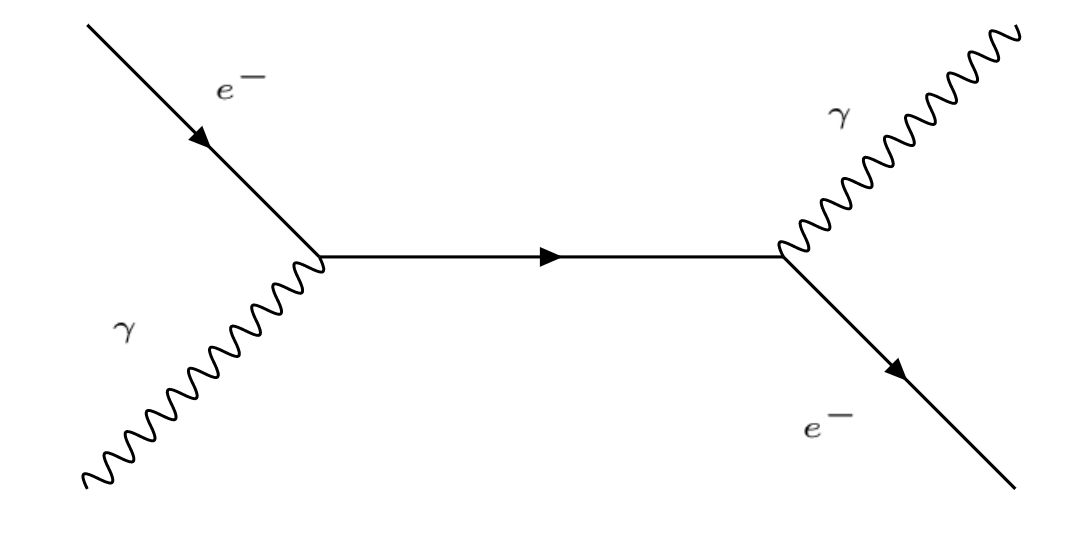
\includegraphics[scale=0.4]{feynman}
\caption{Feynman-Diagramm zur Compton-Streuung (s-Kanal), erstellt mit \cite{feynman}}
\end{figure}
\\\\
Unter den gemachten Bedingungen kann mit Hilfe von Energie- und Impulserhaltung die Energie $E$ der Photonen nach dem Prozess ermittelt werden.
\begin{align}
\label{energiewinkel}
E(\mu) = \frac{E'}{1+ \kappa (1-\mu)}
\end{align}
Hier bei ist $\mu$ der sogenannte Richtungscosinus ($\mu =\cos(\vartheta)$) und $\kappa = \frac{E'}{m_{0}c^2}$.
\\\\
Jetzt können 2 Spezialfälle unterschieden werden:
\begin{itemize}
\item Vorwärtsstreuung: $\mu \rightarrow 1$ und somit $E \rightarrow E'$
\\
\item Rückwärtsstreuung: $\mu \rightarrow -1$ und somit $E \rightarrow \frac{E'}{1+2\kappa}$
\end{itemize}

\subsection{Wirkungsquerschnitt}
Der Wirkungsquerschnitt $\sigma$ macht eine Aussage über die Wechselwirkungswahrscheinlichkeit der Photonen mit Materie. Für die kinematische Betrachtung der Compton-Streuung ist der differentielle Wirkungsquerschnitt $\frac{d\sigma}{d\Omega}$, also der Wirkungsquerschnitt pro Raumwinkelelement $d\Omega = \sin(\vartheta) \, d\vartheta \, d\varphi$, durch die Klein-Nishina-Formel gegeben:
\begin{align}
\label{klein}
\sigma_{\Omega}^{KN}(\mu) = \frac{r_{e}^2}{2} \cdot \left(\frac{1}{1+\kappa(1-\mu}\right)^2 \cdot \left(\kappa(1-\mu)+\frac{1}{1+\kappa(1-\mu)}+\mu^2\right)
\end{align}
$r_{e}$ ist hierbei der klassische Elektronenradius ($r_{e} = 2,818 \cdot 10^{-15}$ m).
\\\\
Aufgrund der Annahme, dass keine Bindungsenergie vorhanden sei, ist der tatsächliche Wirkungsquerschnitt abweichend von $\sigma_{\Omega}^{KN}$. Der differentielle Wirkungsquerschnitt der inkohärenten Streuung $\sigma_{\Omega}^{i}$ ist erst durch Multiplikation mit der inkohärenten Streufunktion $S(E', \mu, Z)$ gegeben:
\begin{align}
\sigma_{\Omega}^{i} = \sigma_{\Omega}^{KN} \cdot  S(E', \mu, Z)
\end{align}
Die Streufunktion $S$ ist also offenbar materialabhängig.

\subsection{Halbleiterdetektoren}
Zur Messung in diesem Versuch wird ein Halbleiterdetektor verwendet, weshalb hier die Funktionsweise eines solchen Detektors zusammengestellt ist.\\\\
Der hier verwendete Detektor ist aus Germanium. Dieser hat eine Bandlücke von $0,67 \, \text{eV}$. Durch die auftreffenden Photonen können Elektronen diese Bandlücke überwinden und stehen als Ladungsträger im Leitungsband zur Verfügung. Für Germanium wird dazu lediglich eine Photonenenergie von $2,8$ eV benötigt.
\\\\
Ultrareine Detektoren können ja nach Restverunreinigung als $\pi$- oder $\nu$- Typ klassifiziert werden. Hier ist das Schema eines solchen planaren HP-Ge-Detektors:
\begin{figure}[h!]\centering
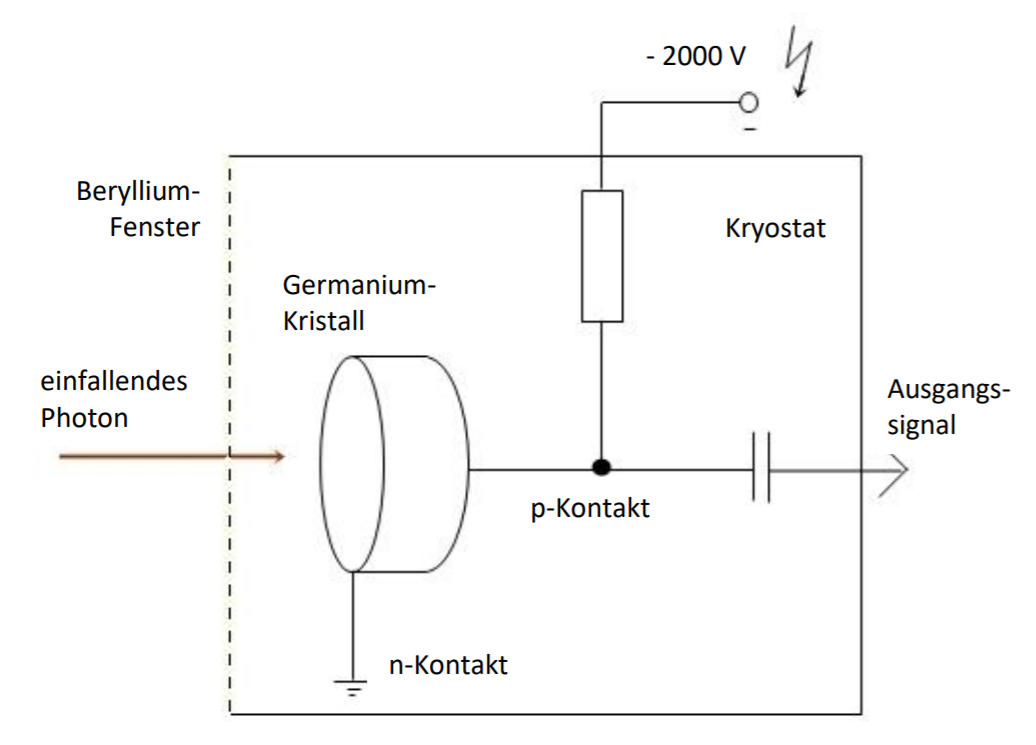
\includegraphics[scale=0.4]{detektor}
\caption{Schema eines planaren HP-Ge-Detektors, entnommen aus \cite{Anleitung}}
\end{figure}
\newpage
Der fensterseitige Außenkontakt hat für einen $\pi$-Typ eine $100 \, \mu$m dicke $\text{n}^{+}$-Dotierung und für einen $\nu$-Typ eine 0,1 $\mu$m dicke $\text{p}^{+}$-Dotierung. Dabei sind die Kontakte eine nicht zum aktiven Volumen des Detektors beitragende Totschicht. Da der Außenkontakt des $\nu$-Typs so dünn ist, ist er gut zur Detektion niederenergetischer Photonen geeignet. Es ist zu beachten, dass diese Detektoren allerdings mit flüssigem Stickstoff gekühlt werden müssen, um das thermische Rauschen zu unterbinden. Die Dicke des Kristall beträgt etwa $5$ bis $20$ mm und die Ansprechwahrscheinlichkeit des Detektors für Strahlung im Bereich von einigen keV bis $80$ keV ist nahezu $100$\%.

\section{Versuchsaufbau}
Der verwendete Versuchsaufbau ist in folgendem Bild gegeben:
\begin{figure}[h!]\centering
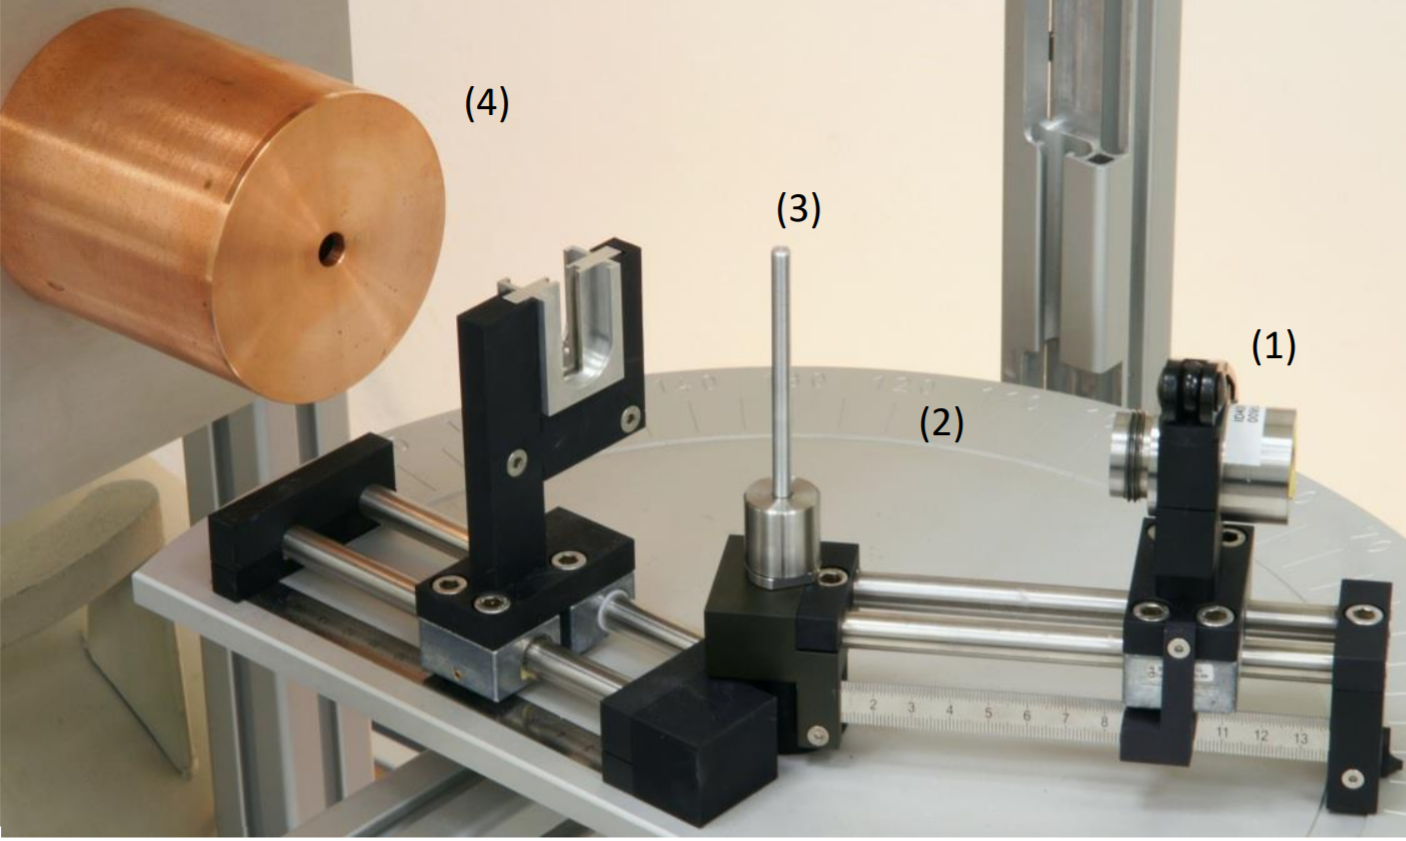
\includegraphics[scale=0.4]{aufbau}
\caption{Verwendeter Versuchsaufbau, entnommen aus \cite{Anleitung}}
\end{figure}
\\
Die einzelnen Komponenten sind dabei durchnummeriert:
\begin{itemize}
\item (1) beweglicher Halter 
\item (2) Goniometer zur Einstellung des Winkels ($0^{\circ} \leq \vartheta \leq 170^{\circ}$)
\item (3) Streukörper (Stabe unterschiedlicher Dicke und Materialien)
\item (4) Detektor (Halbleiterdetektor)
\end{itemize}

\section{Durchführung}

\begin{itemize}
\item Kalibrierung: Aufnahme der Impulshöhenverteilung für verschiedene spektrometrische Quellen und linearer Fit der Maxima bekannter Energien zur Erstellung der Kalibriergerade
\item Aufnahme eines Histogramms für eine $^{241}$Am-Quelle mit $\vartheta = 90^{\circ}$ und einem Aluminiumstreustab der Dicke $d=8$ mm für $t = 20$ min
\item Zeitoptimierung: Messung für die $^{241}$Am-Quelle mit $\vartheta = 90^{\circ}$ ohne Streukörper und Ermittelung der optimalen Messzeit $t_{\text{opt}}$
\item Bestimmung der Energie gestreuter Photonen: Messung der Energie gestreuter Photonen für unterschiedliche Winkel $\vartheta$: $30^{\circ}, 45^{\circ}, 60^{\circ}, 75^{\circ}, 90^{\circ}, 105^{\circ}, 120^{\circ}, 130^{\circ}$
\item Bestimmung des Wirkungsquerschnitts: Graphische Darstellung des Messergebnisses und $\sigma_{\Omega}^{KN}$ über $\mu = \cos(\vartheta)$
\item Einfluss des Streukörperdurchmessers: Aufnahme von Histogrammen für den minimalen Abstand zwischen Quelle und Streukörper bei $\vartheta= 60^{\circ}$ und graphische Darstellung der Zählrate $\dot{N}$ in Abhängigkeit vom Streukörperdurchmesser $d$
\item Einfluss des Abstands zwischen Quelle und Streukörper: Untersuchung der Änderung des Messeffekts in Abhängigkeit des Abstands $l$ bei festem $\vartheta = 60^{\circ}$ und festem $d= 6$mm
\end{itemize}

\section{Auswertung}

\subsection{Kalibrierung}
Zur Energiekalibrierung wurden folgende Proben verwendet: $^{152}$Eu, $^{137}$Cs und $^{133}$Ba. Diese Spektren wurden also vermessen und sind im Folgenden dargestellt. Die Anzahl der Zählungen (Counts) sind über dem jeweiligen Kanal dargestellt. Es wurde zudem jeweils für 2 Peaks ein Gauß-Fit durchgeführt, um die Kanallage zu bestimmen und dazu eine Unsicherheit zu erhalten. In der graphischen Darstellung ist jeweils blau das tatsächlich gemessene Spektrum und rot der Gauß-Fit der Peaks:
\begin{figure}[h!]\centering
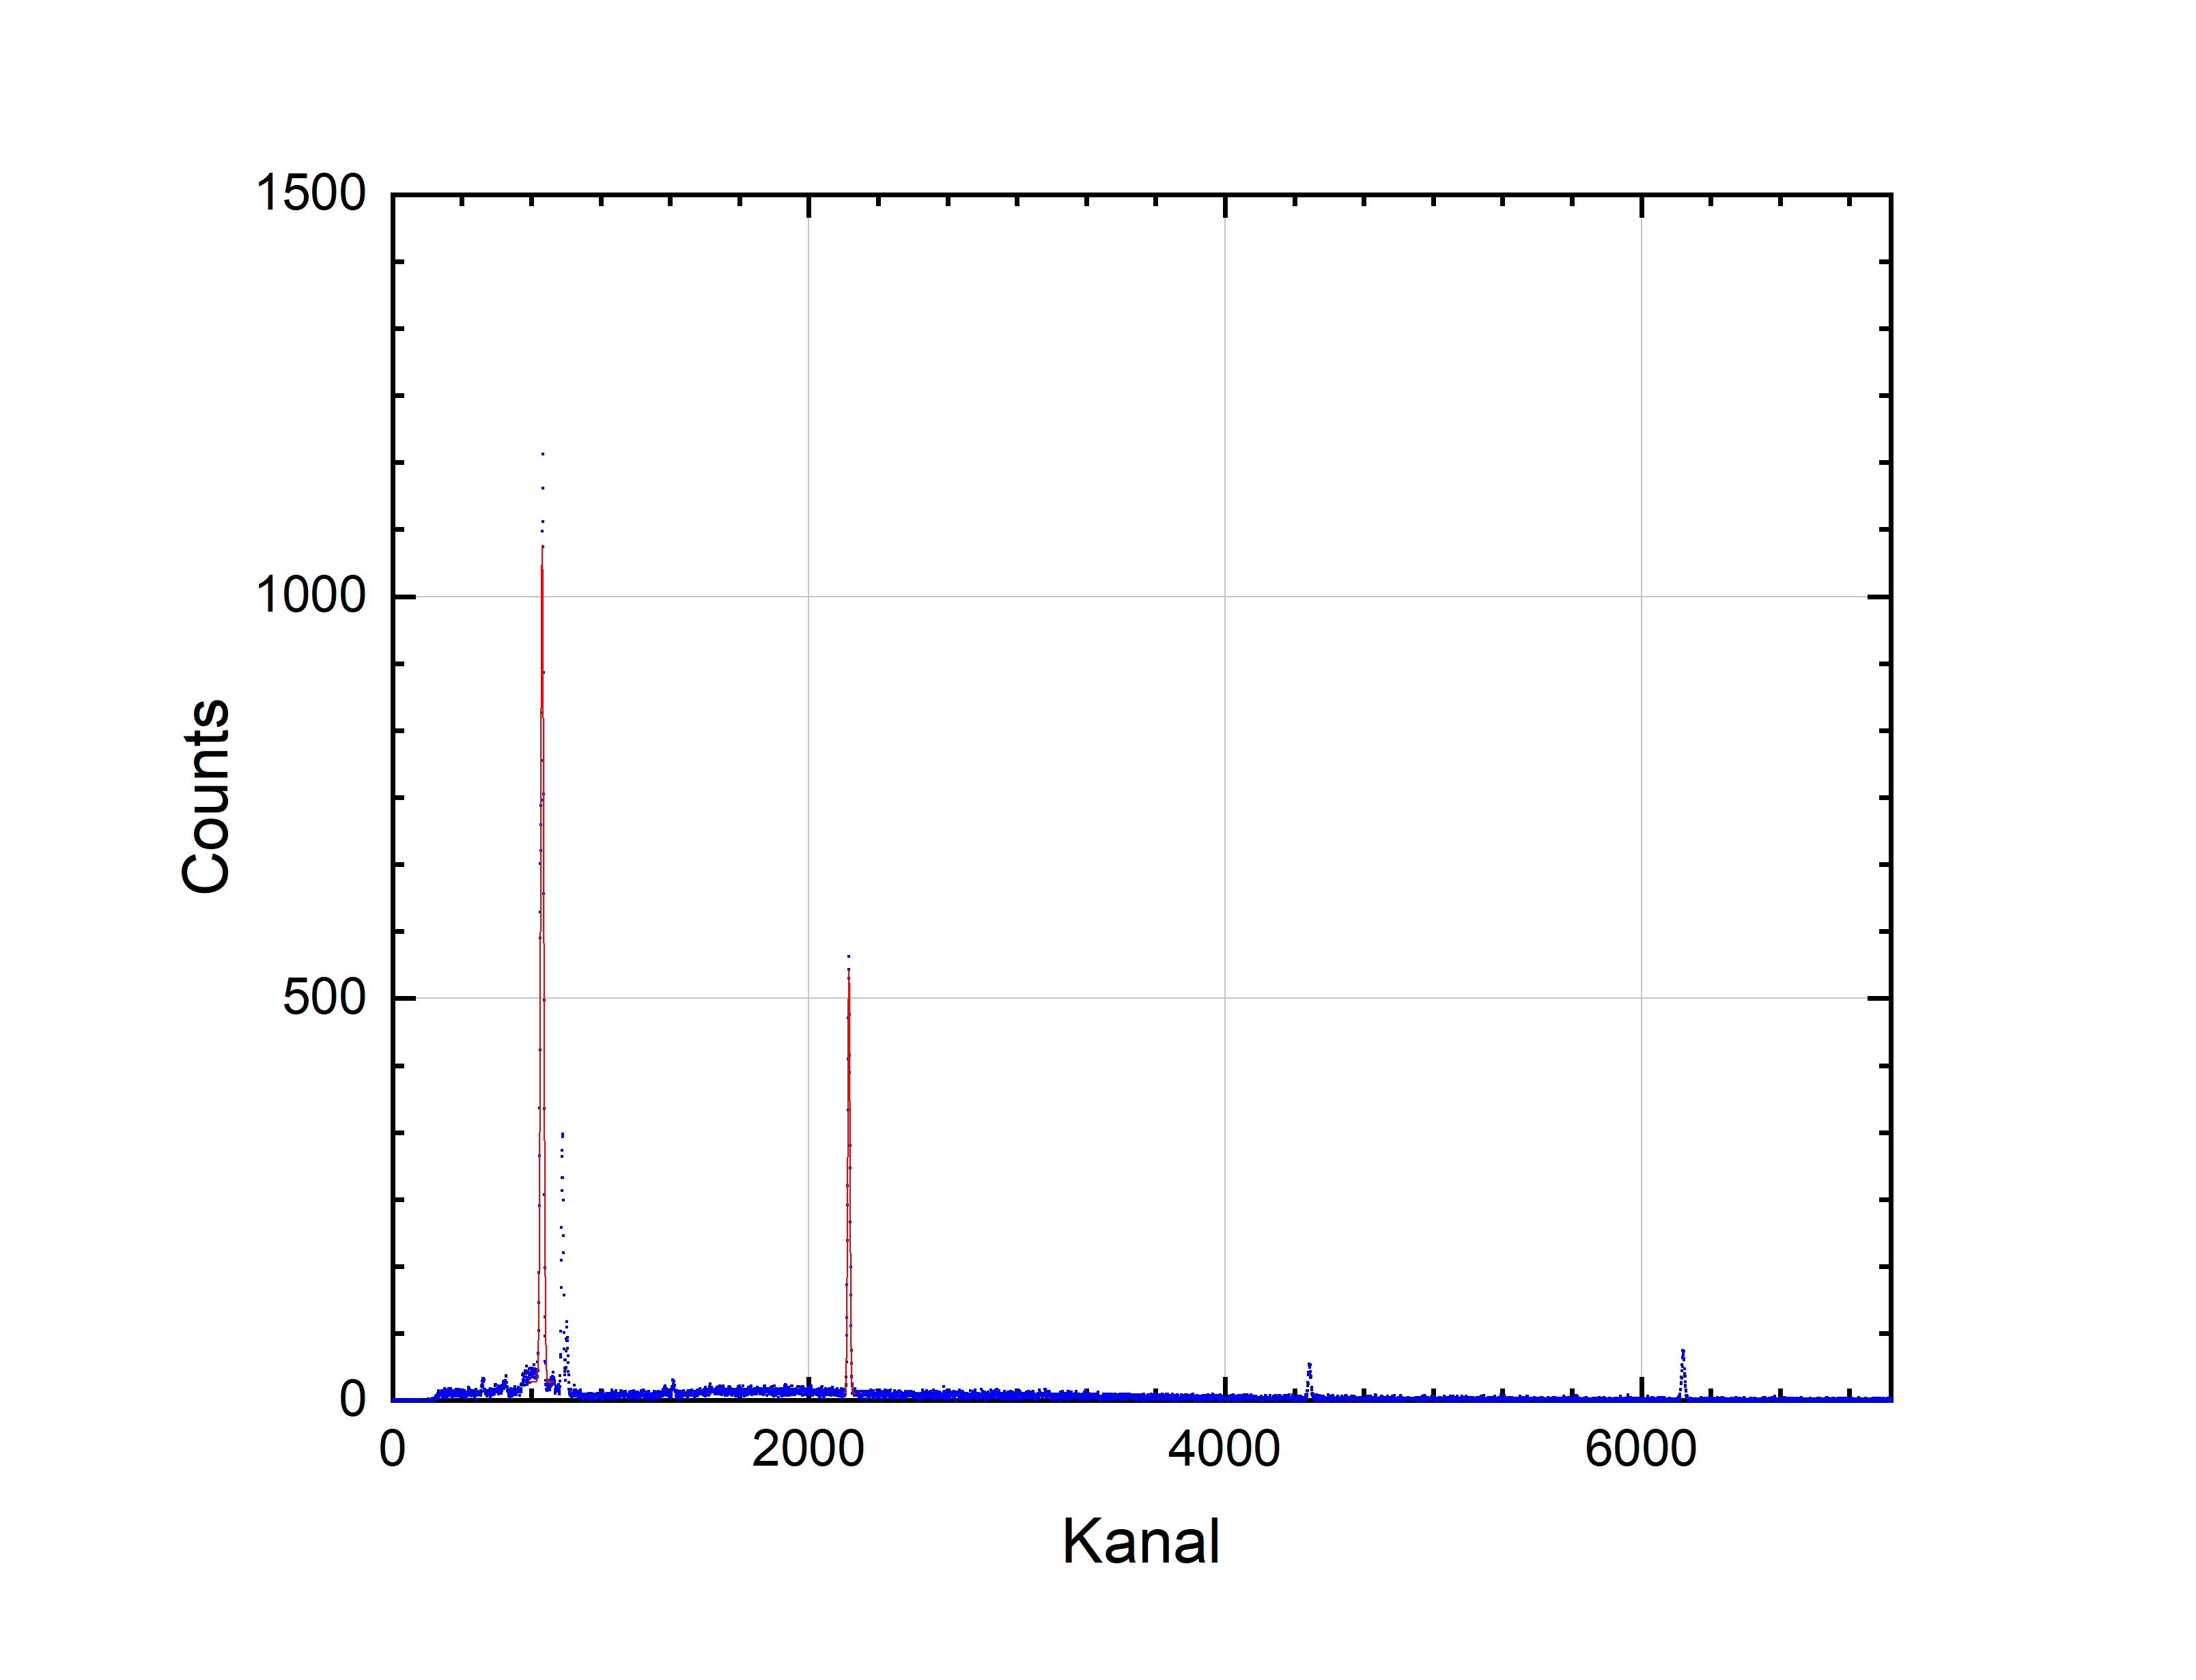
\includegraphics[scale=0.43]{Europium_Peaks}
\caption{Spektrum für $^{152}$Eu mit Gauß-Fit von zwei Peaks}
\end{figure}
\newpage
\begin{figure}[h!]\centering
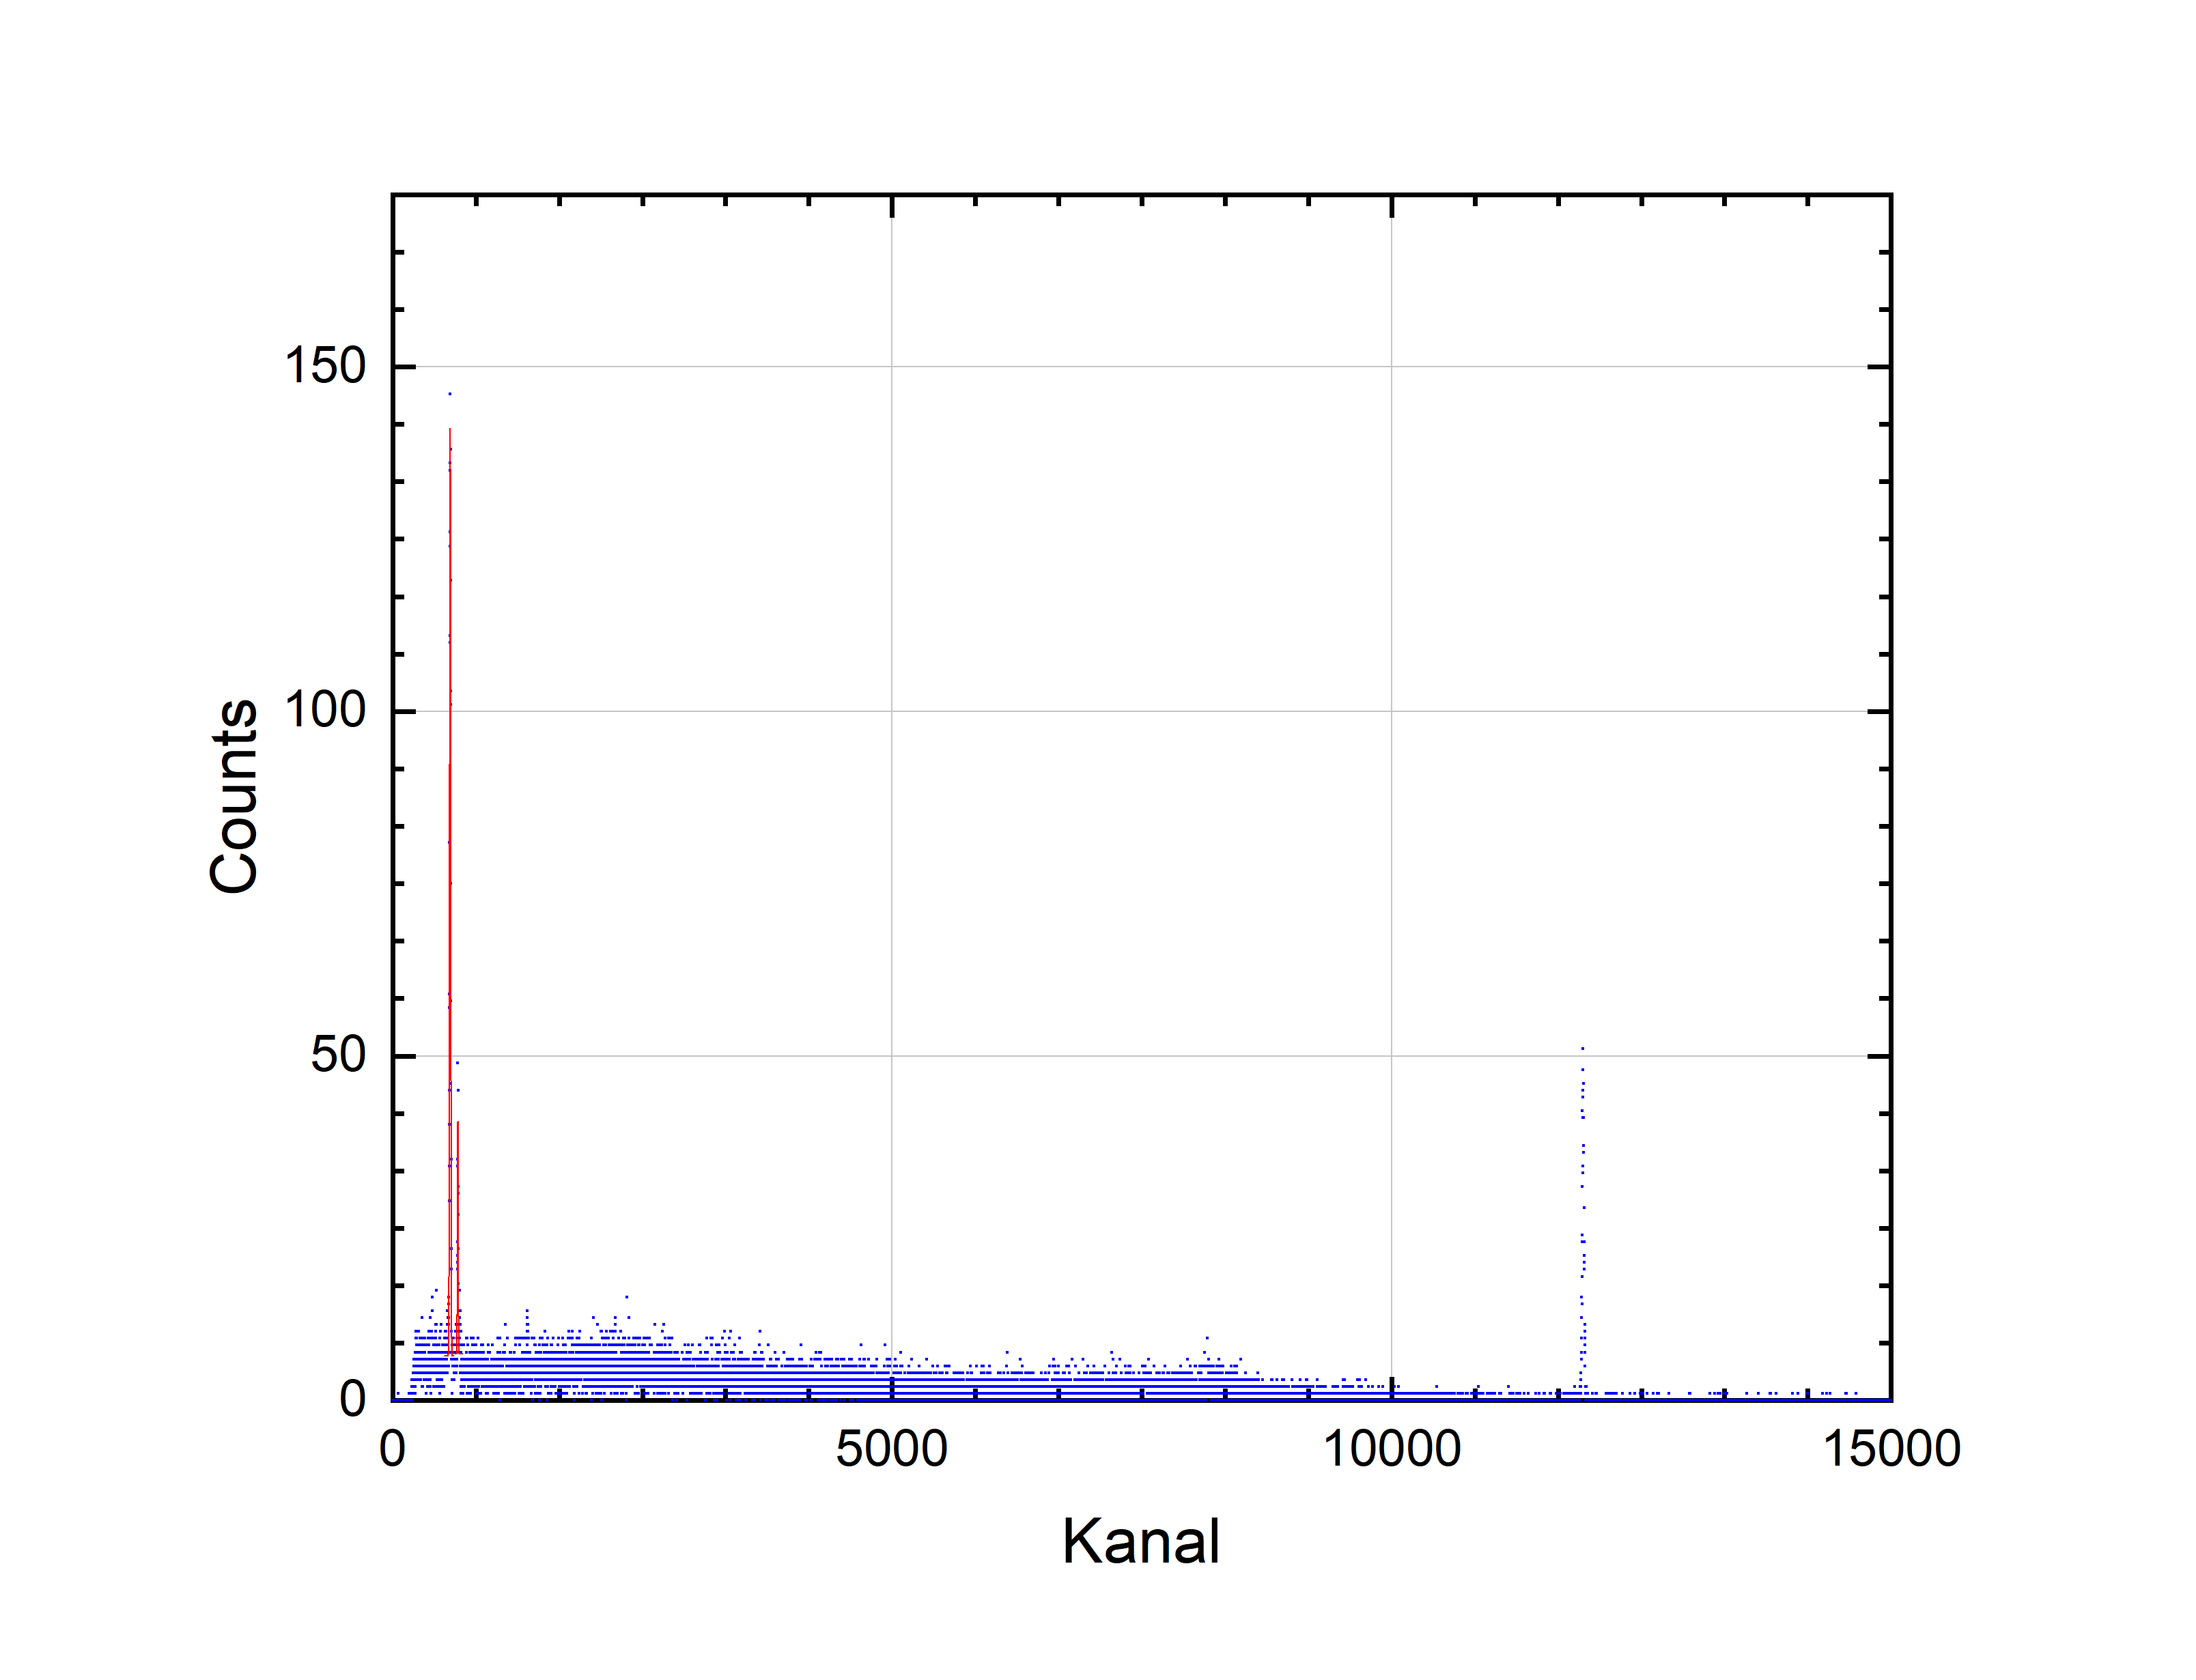
\includegraphics[scale=0.43]{Caesium_Peaks}
\caption{Spektrum für $^{137}$Cs mit Gauß-Fit von zwei Peaks}
\end{figure}
\begin{figure}[h!]\centering
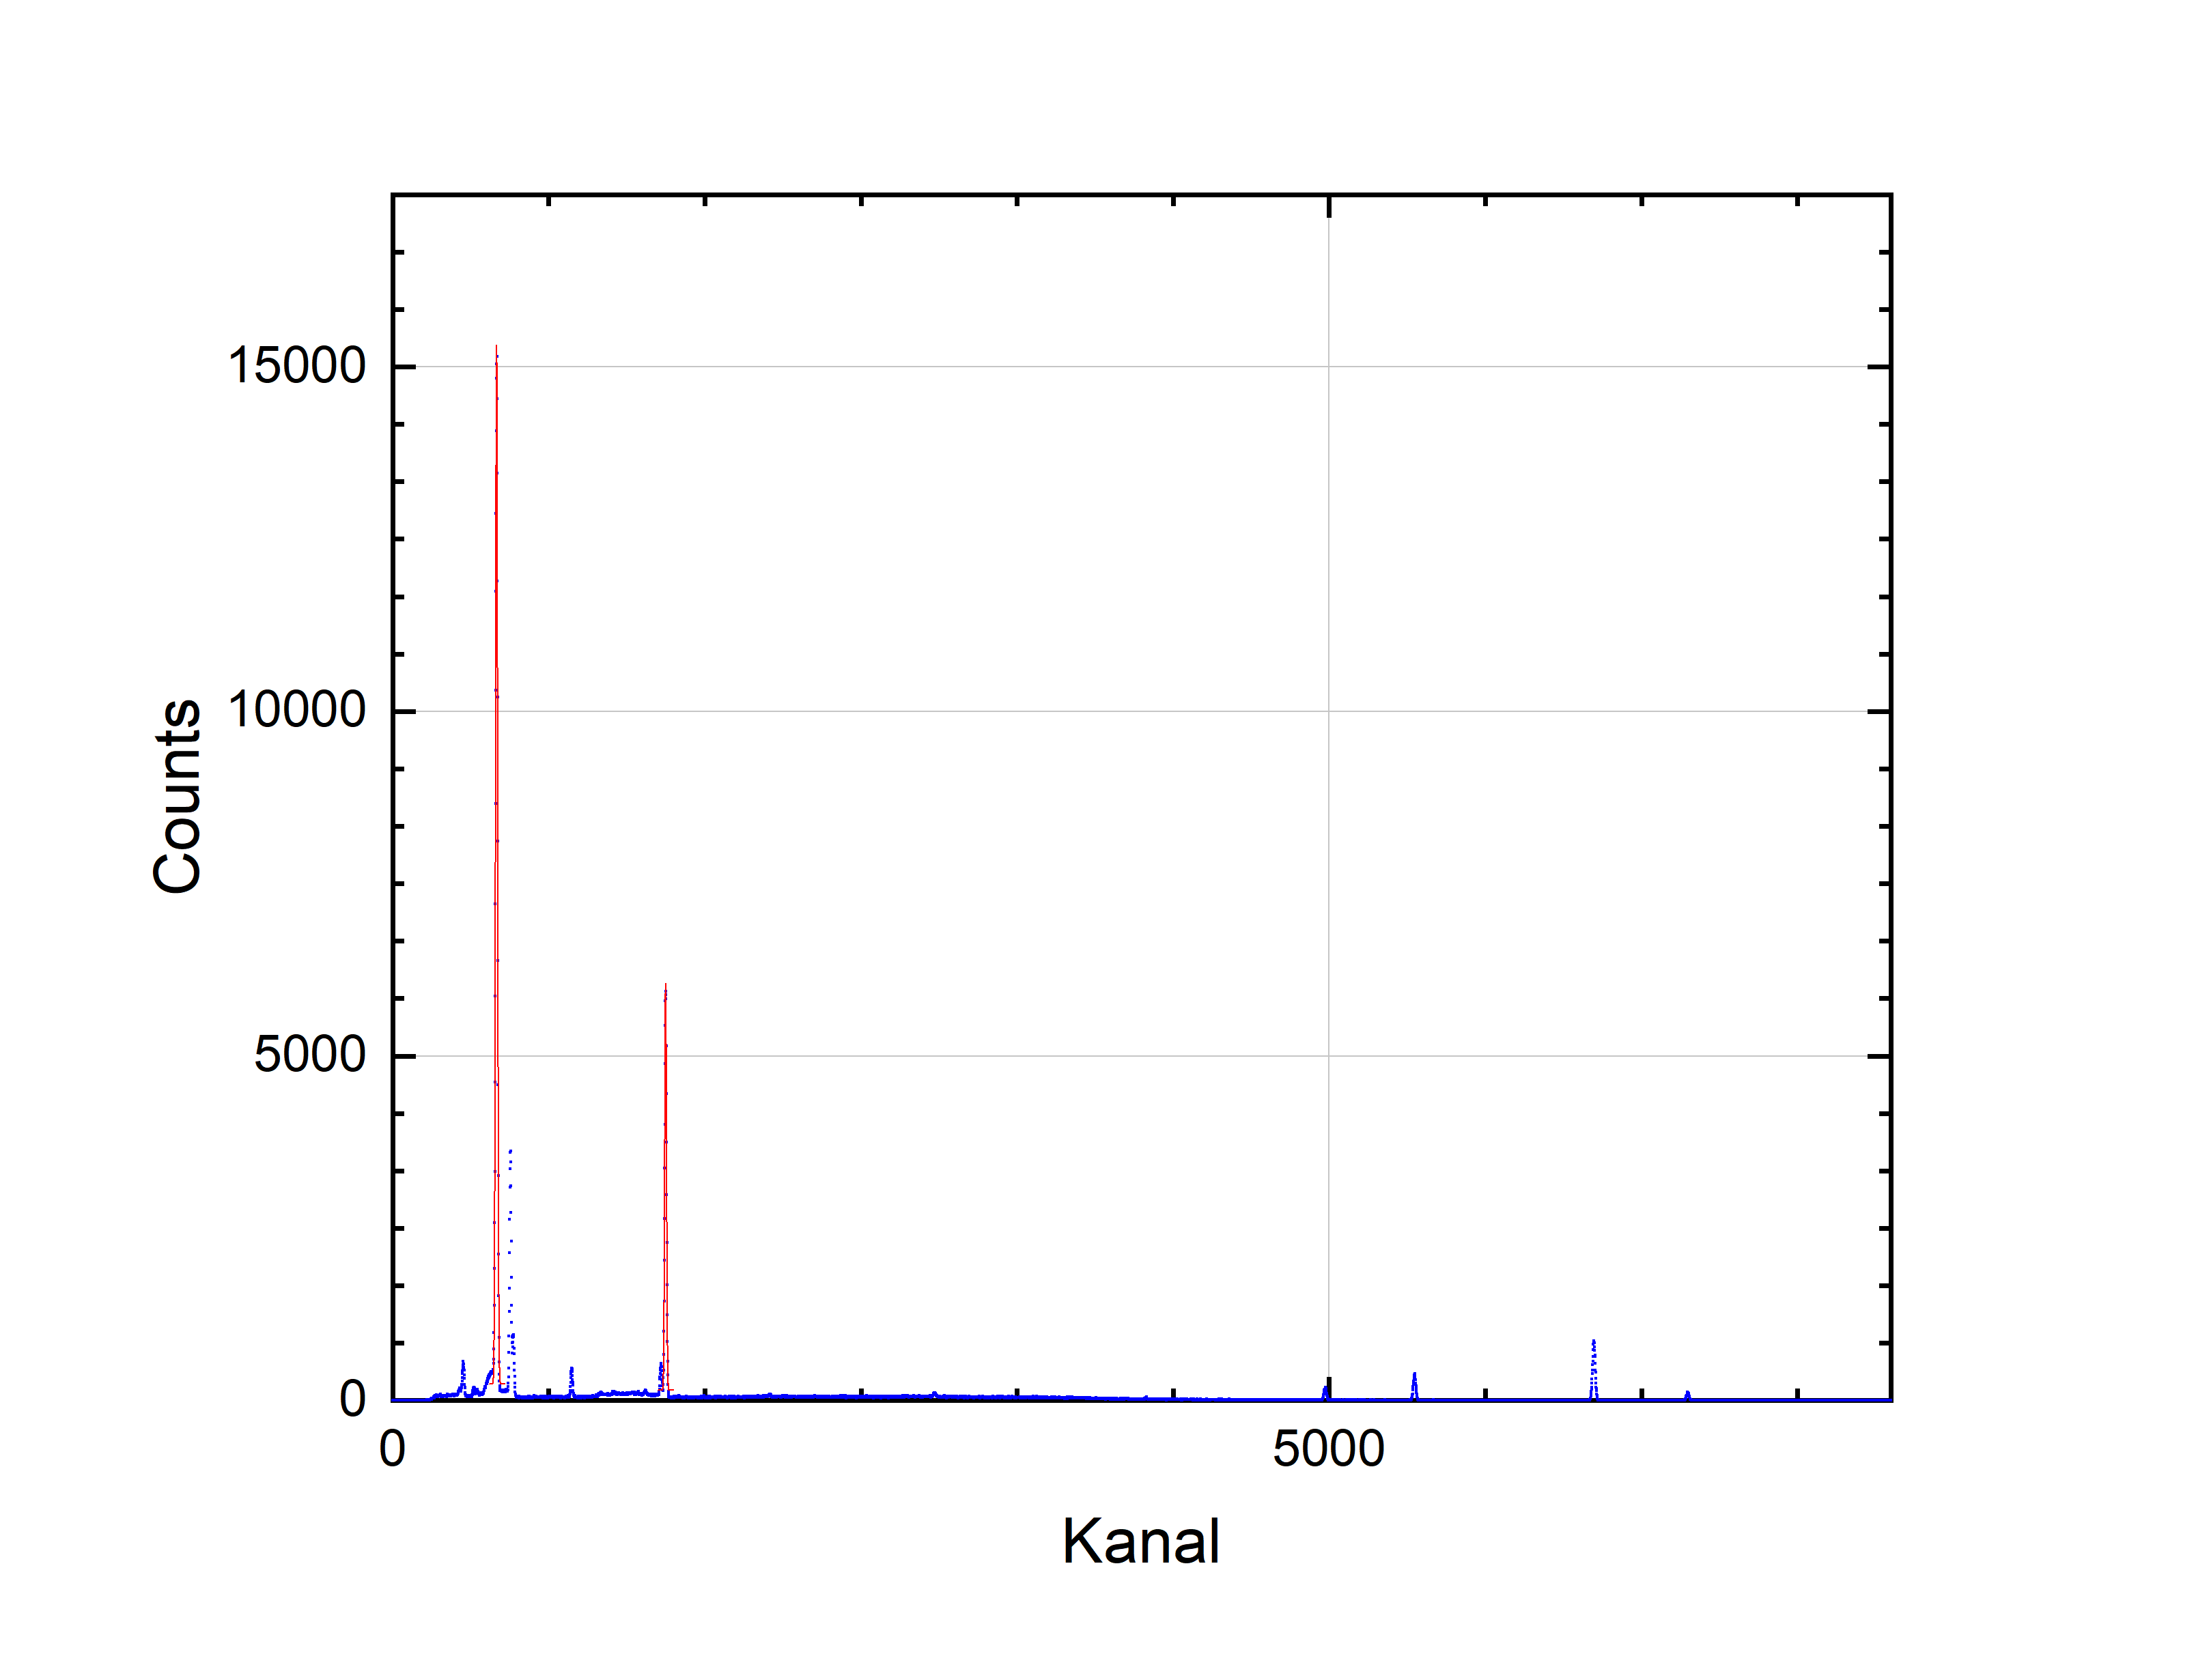
\includegraphics[scale=0.43]{Barium_Peaks}
\caption{Spektrum für $^{133}$Ba mit Gauß-Fit von zwei Peaks}
\end{figure}
\newpage
Der so ermittelte Kanal mit Fehler musste nur noch einer gewissen Energie zugeordnet werden. Dazu wurde die Website NuDat (\cite{nudat}) verwendet. Somit ergab sich folgende Tabelle:
\\\\
\begin{table}[h!]\centering
\begin{tabular}{|c|c|c|c|}\hline
Probe & Kanallage des Peaks & Fehler Kanallage des Peaks & (Energie des Peaks)/keV \\\hline
$^{152}$Eu & 719,20 & 0,17 & 39,522 \\\hline
$^{152}$Eu & 2192,80 & 0,04 & 121,7817 \\\hline
$^{137}$Cs & 577,61 & 0,07 & 31,817 \\\hline
$^{137}$Cs & 654,37 & 0,22 & 32,194 \\\hline
$^{133}$Ba & 555,81 & 0,04 & 30,973 \\\hline
$^{133}$Ba & 1458,26 & 0,05 & 80,9979 \\\hline
\end{tabular}
\caption{Zuordnung Energie und Kanal der Kalibrierproben}
\end{table}
\\\\
Nun konnten diese Werte in einem neuen Diagramm eingetragen werden, um einen linearen Fit vorzunehmen und so die Geradengleichung zu erhalten. Dabei sind die Fehler für die Energie allerdings nicht zu erkennen, da diese zu klein sind (die Peaks im Spektrum waren also dementsprechend scharf).
\newpage
\begin{figure}[h!]\centering
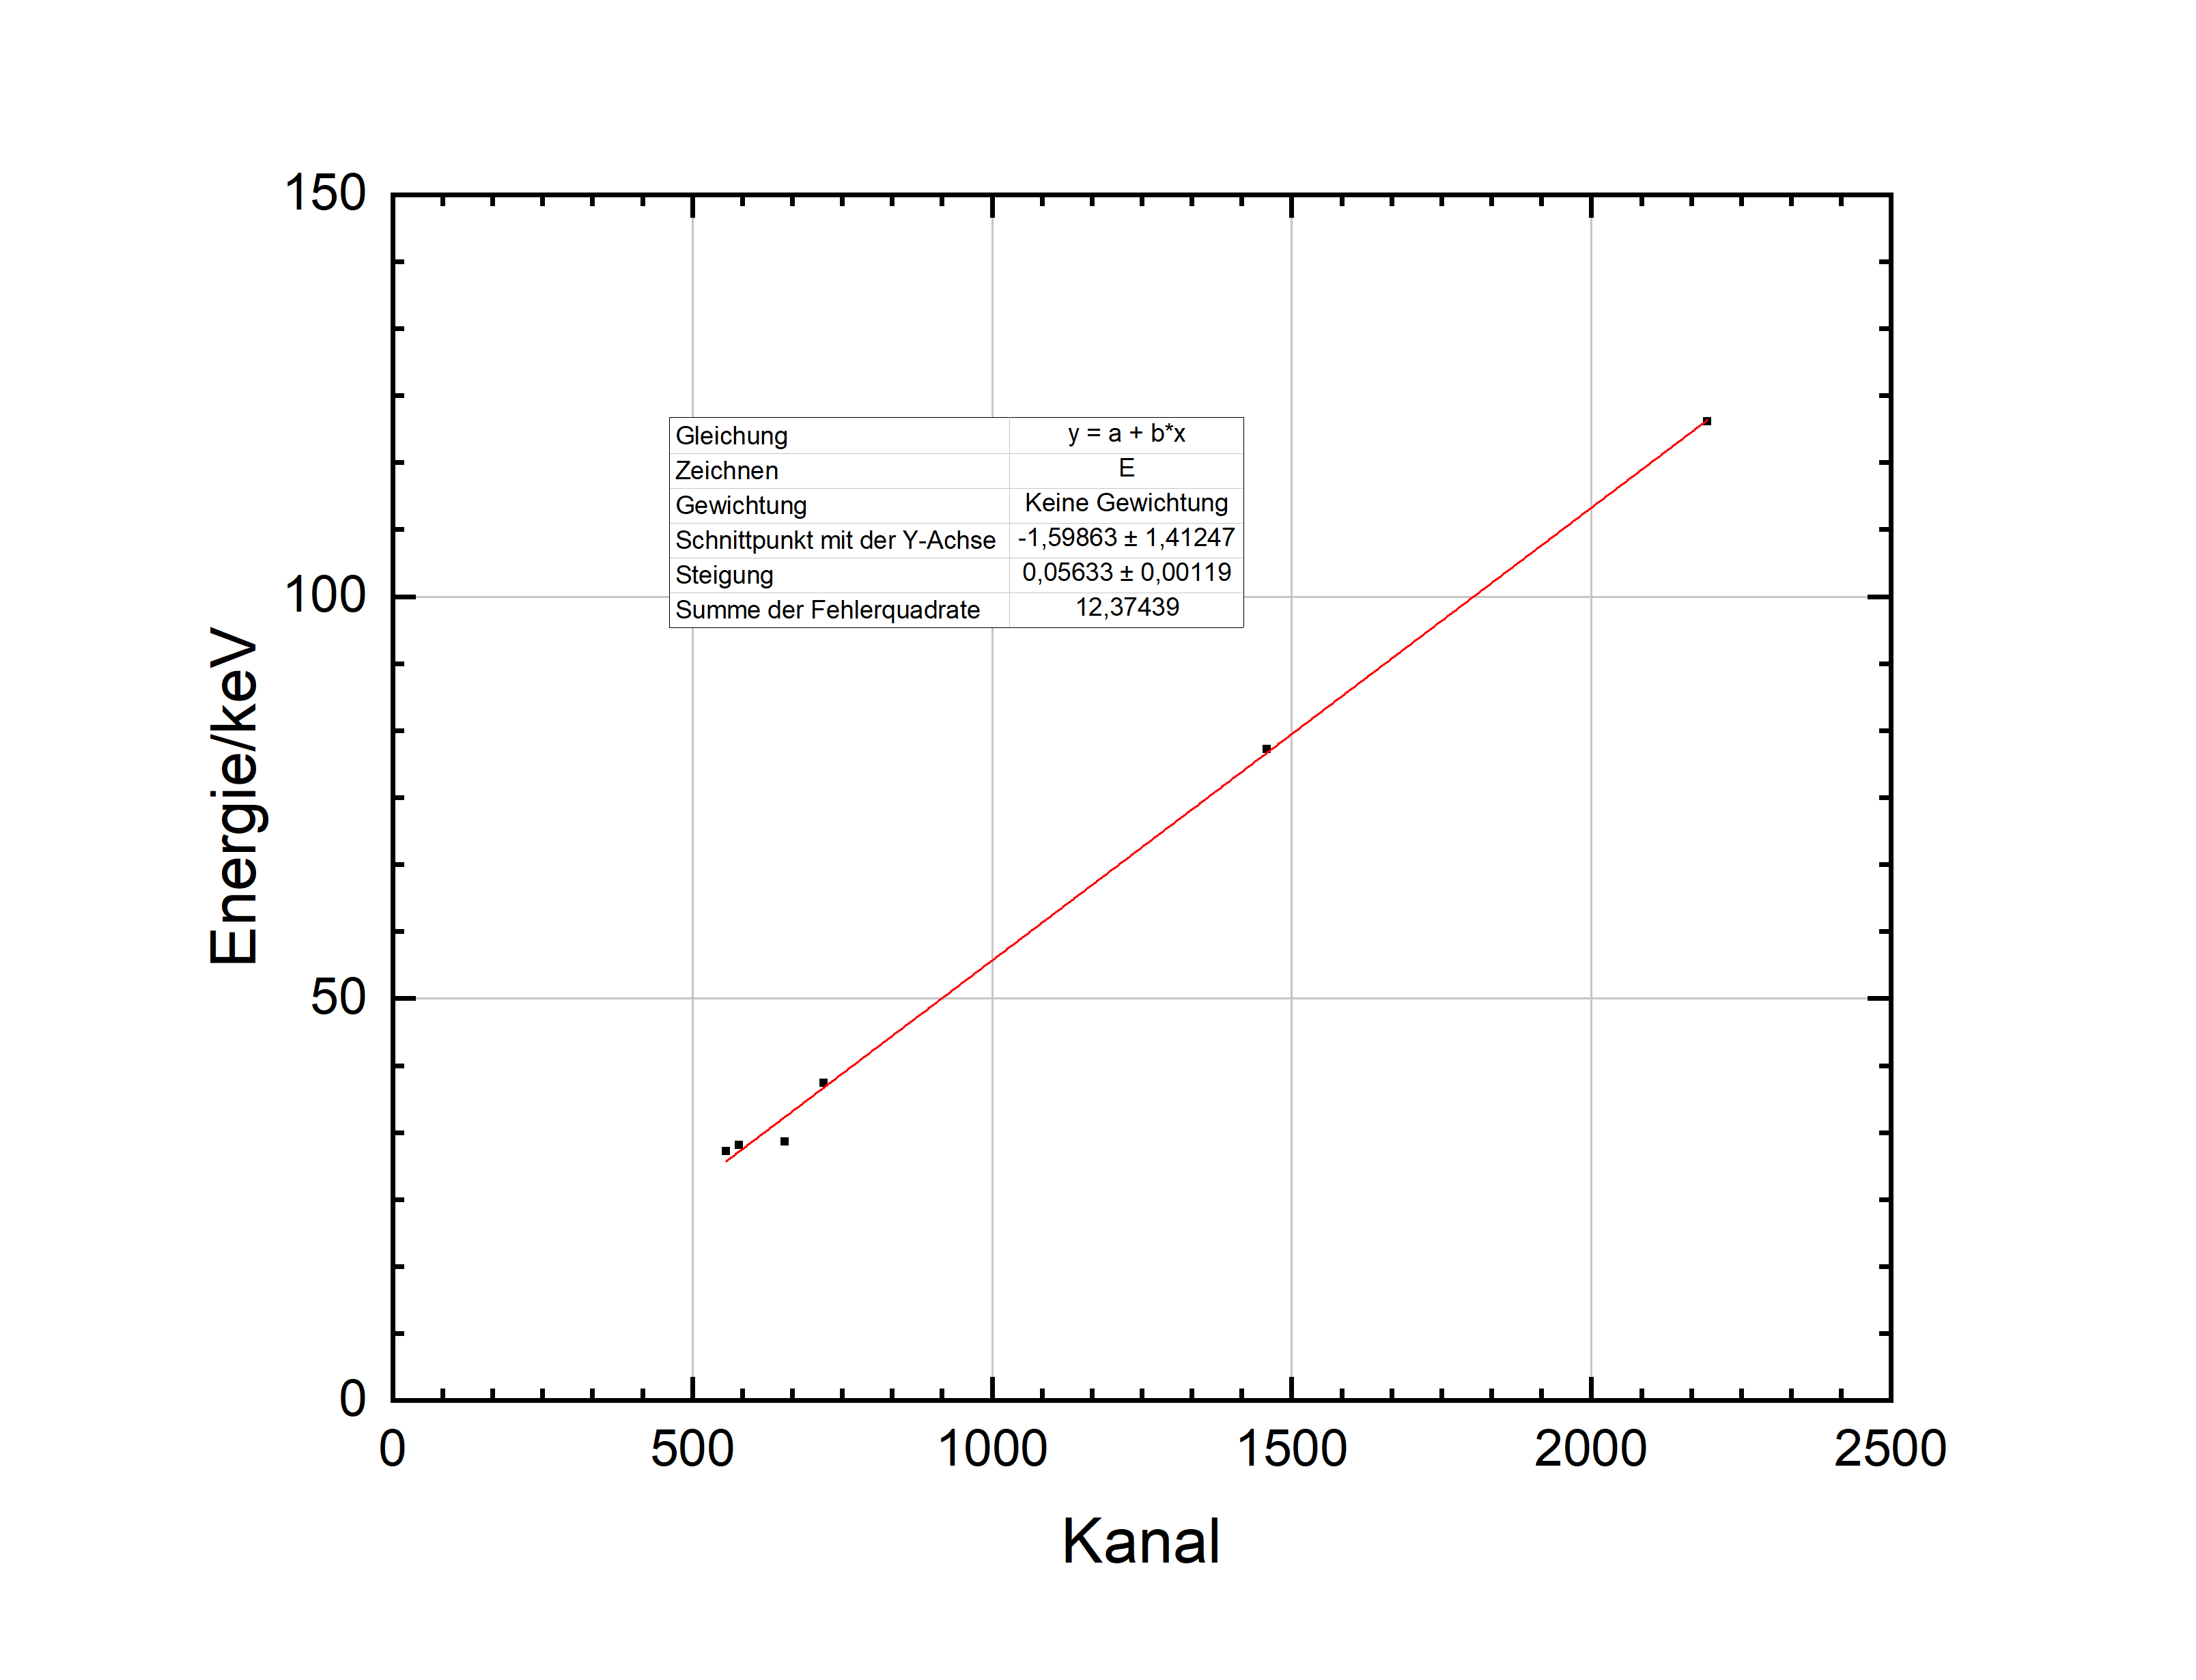
\includegraphics[scale=0.6]{kalibrierung}
\caption{Linearer Fit (Kalibriergerade)}
\end{figure}
Zusammenfassend wurde also folgende Geradengleichung für die Kalibriergerade gefunden:
\begin{align}
E(K) = -1,59863 \,  \text{keV} + 0,05633 \, \text{keV} \cdot K
\end{align}
Diese Gleichung ermöglicht es jetzt also gemessene Energien, also deren Kanallage, in die Einheit keV umzurechnen.
\newpage

\subsection{Aufnahme eines Histogramms}
Es galt hier für den Streustab aus Aluminium ein Histogramm aufzunehmen. Abweichend von der originalen Anleitung wurde hier ein Streustab der Dicke $d=8$\,mm verwendet. Außerdem wich die Messzeit um ein paar Sekunden von den gegebenen $20$ min ab. Allerdings wurde die tatsächliche Messzeit nicht notiert. Dies sollte aber unter Berücksichtigung dieser geringen Abweichung von ca. $3$\,s...$5$\,s im Vergleich zu den $20$ min keinen großen Einfluss haben. Das Histogramm ist hier zu sehen:
\\\\
\begin{figure}[h!]\centering
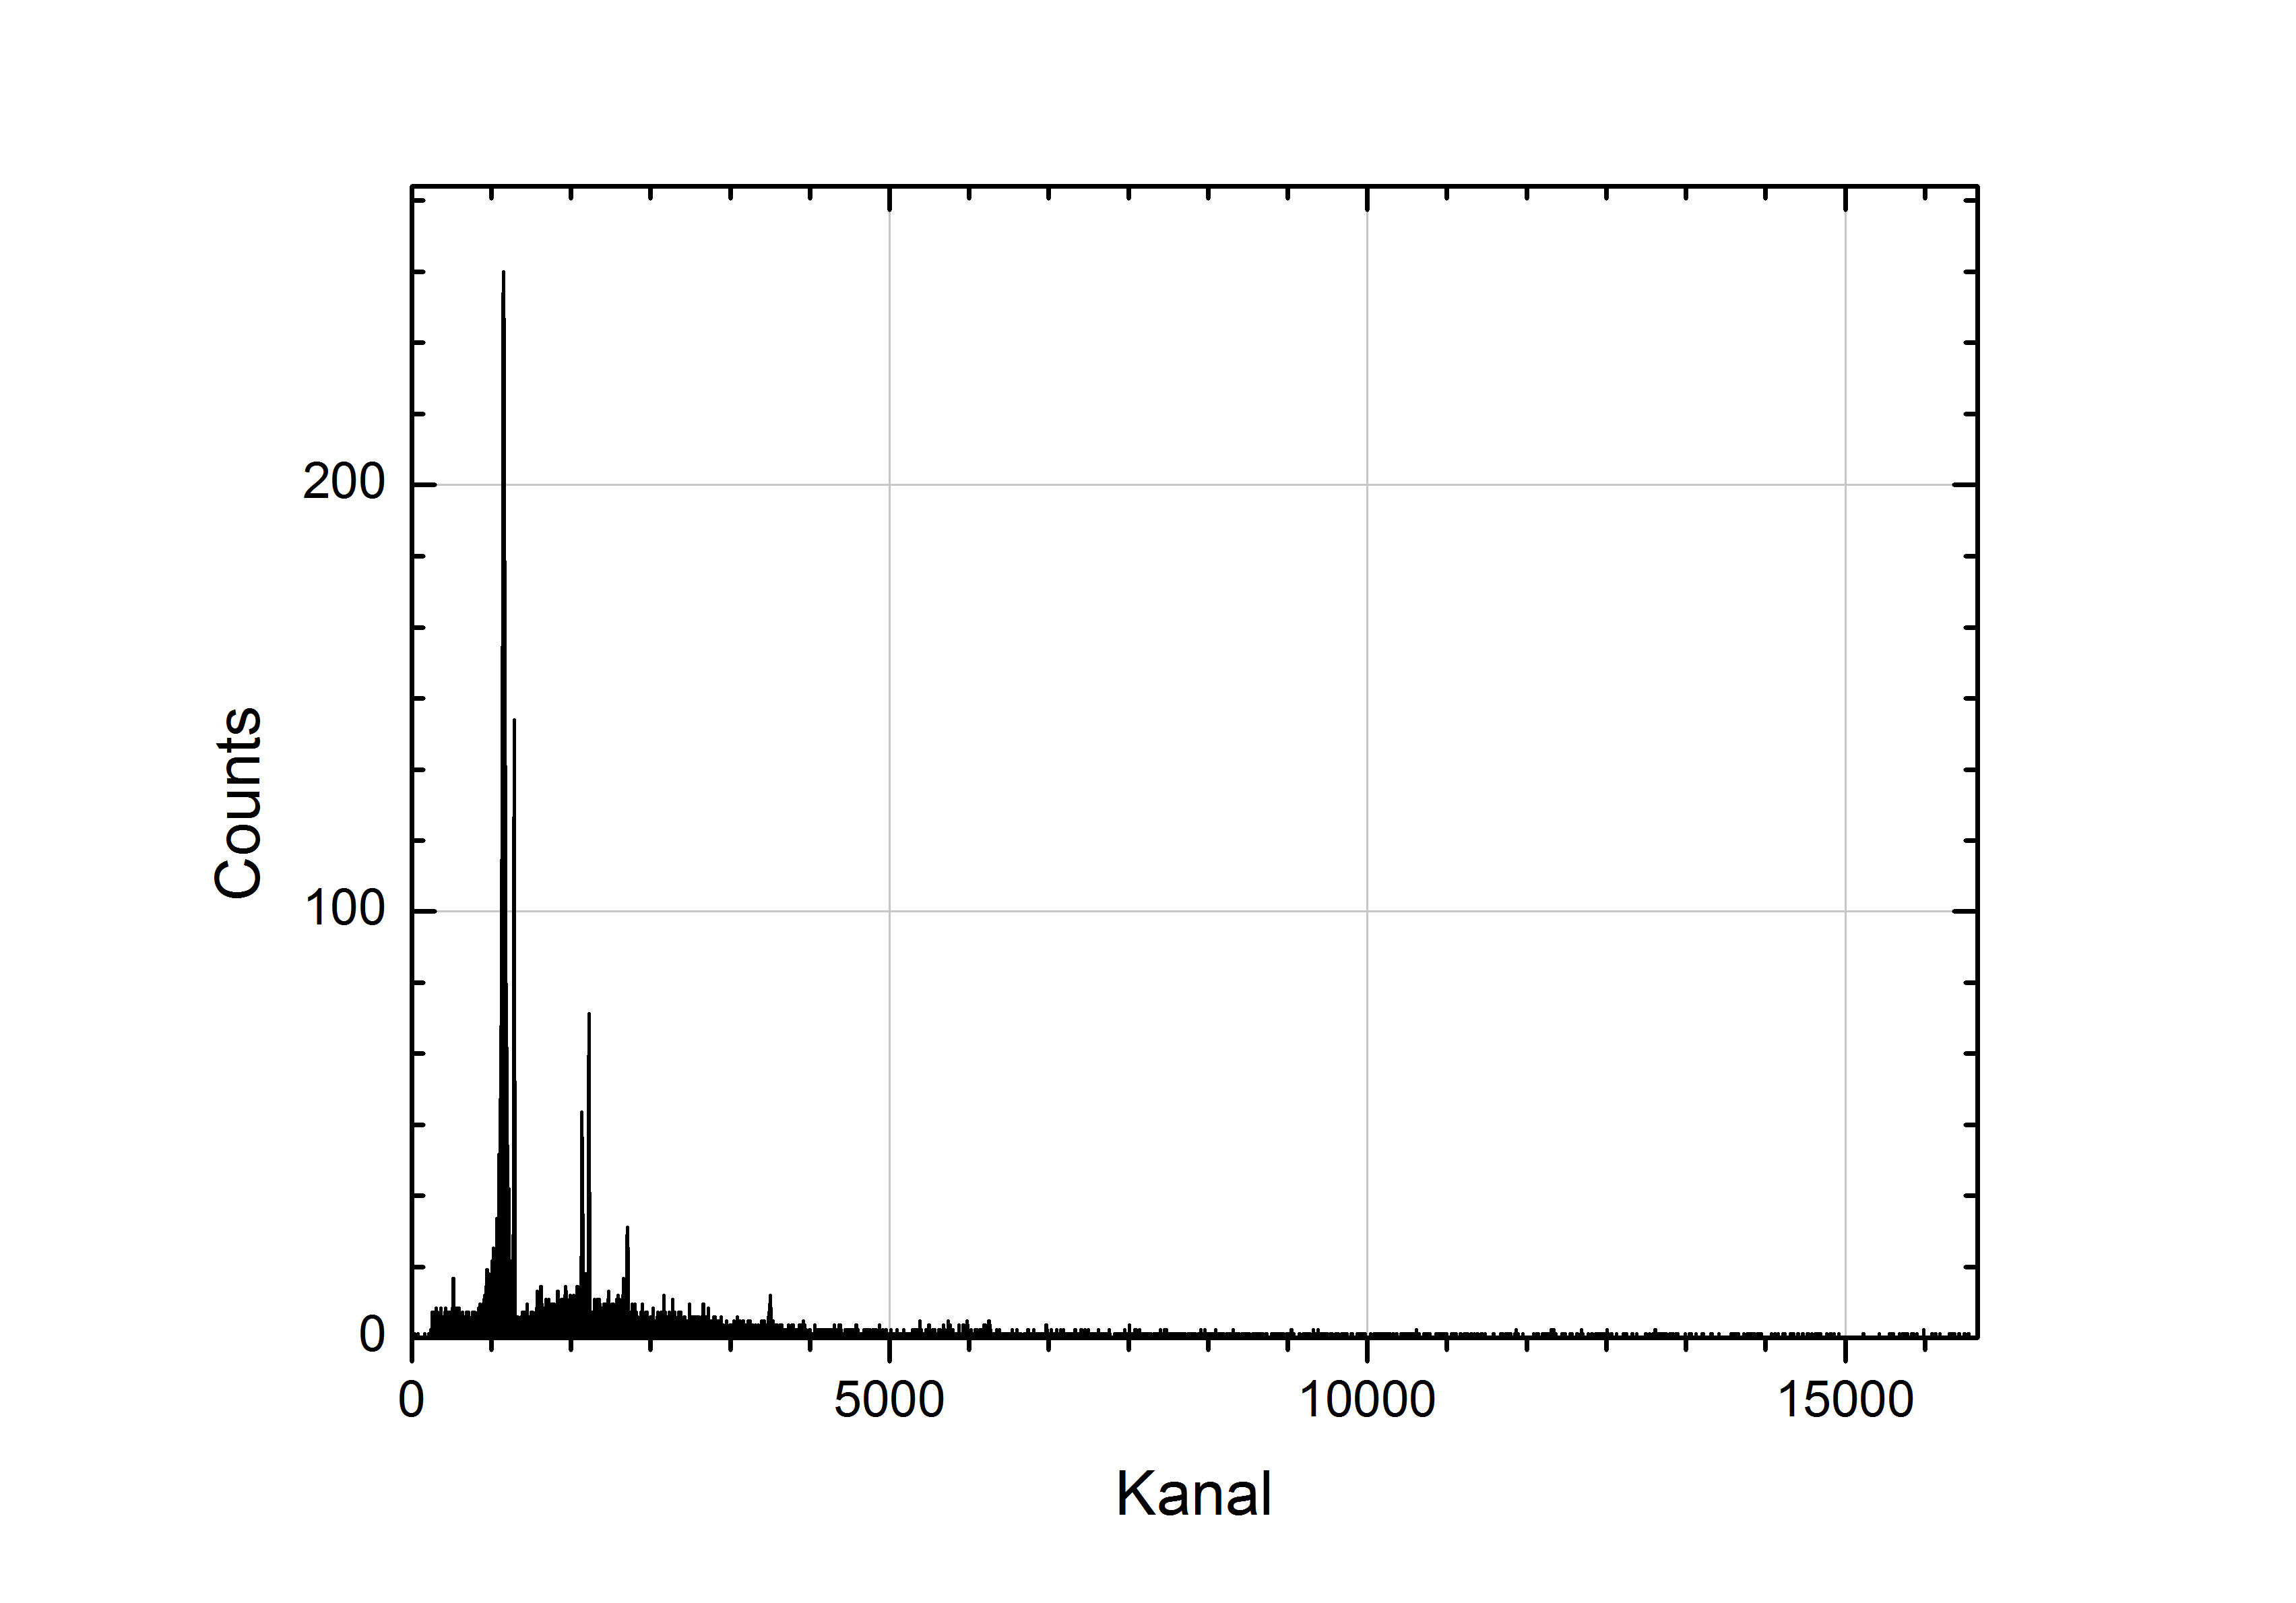
\includegraphics[scale=0.5]{histogramm}
\caption{Histogramm für $^{241}$Am-Quelle, $\vartheta=90^{\circ}$, $t_{\text{mess}}$\,=\,$20$ min}
\end{figure}
\\\\
Hier ergeben sich 4 sehr markante Peaks. Deren Kanallage wurde wieder durch einen Gauß-Fit ermittelt und mit Hilfe der Kalibriergerade in eine Energie in keV umgerechnet. Daraus folgt folgende Tabelle:
\newpage
\begin{table}[h!]\centering
\begin{tabular}{|c|c|c|c|}\hline
Kanallage $K$ des Peaks & $\Delta$K& (Energie $E$ des Peaks)/keV & ($\Delta$E)/keV \\\hline
961,71 & 0,22 & 52,57 & 1,81 \\\hline
1371,04 & 0,12 & 58,73 & 1,90 \\\hline
1781,66 & 0,17 & 98,76 & 2,55 \\\hline
1819,89 & 0,27 & 100,92 & 3,00 \\\hline
\end{tabular}
\caption{Kanallage und Energie der 4 markantesten Peaks}
\end{table}
Der Fehler der Kanallage des Peaks wurde wieder aus einem Gauß-Fit bestimmt. Der Fehler der Energie folgt durch Gauß'sche Fehlerfortpflanzung aus den Unsicherheiten der Parameter der Kalibriergerade und der Unsicherheit der Kanallage $K$:
\\
\begin{align*}
\Delta E &= \sqrt{\left ( \frac{\partial E}{\partial a} \, \Delta a \right)^2 + \left (\frac{\partial E}{\partial b} \, \Delta b \right)^2+ \left( \frac{\partial E}{\partial K} \, \Delta K \right)^2} \\\\
\Delta E &= \sqrt{(\Delta a)^2 + (K \, \Delta b)^2 + (b \, \Delta K)^2}
\end{align*}
\\
Jetzt können diese Energien verschiedenen Übergängen des $^{241}_{95}$Am zugeordnet werden. 
\newpage
Dazu wird folgendes Zerfallsschema betrachtet:
\\\\
\begin{figure}[h!]\centering
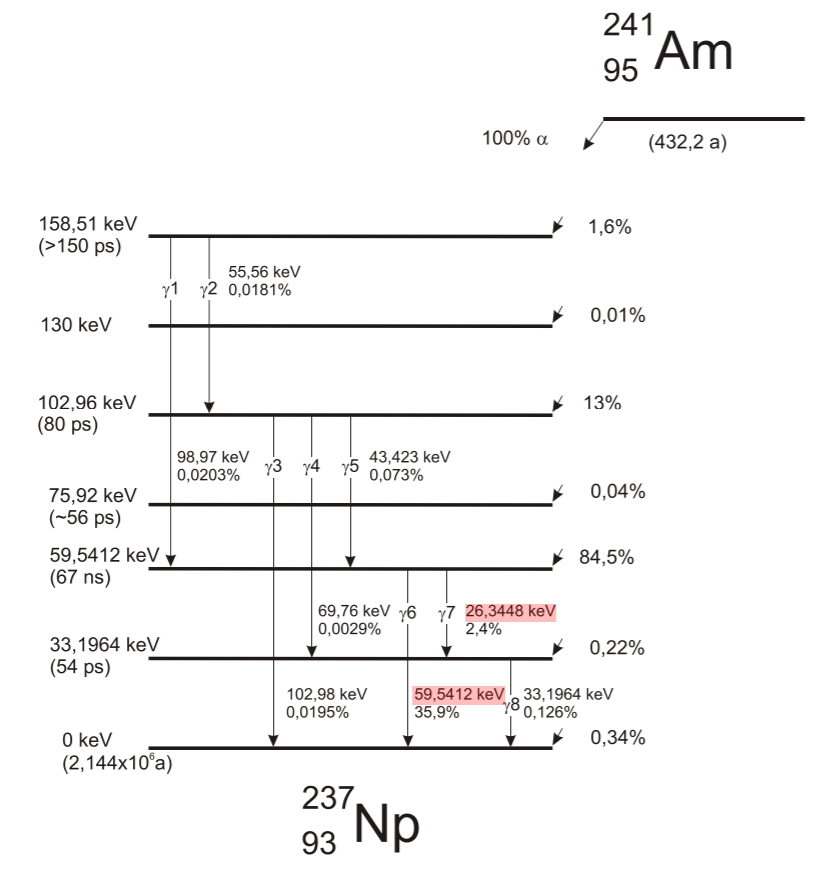
\includegraphics[scale=0.5]{zerfallsschema}
\caption{Zerfallsschema von $^{241}_{95}$Am, entnommen aus \cite{Anleitung}}
\end{figure}
\\\\
Im Rahmen der berechneten Unsicherheit kann also folgende Zuordnung der Peaks zu den Übergängen vorgenommen werden:
\\
\begin{table}[h!]\centering
\begin{tabular}{|c|c|}\hline
(gemessene Energie $E$ des Peaks)/keV & Übergang im Zerfallsschema \\\hline
52,57 & $\gamma_{2}$ \\\hline
58,73 & $\gamma_{6}$ \\\hline
98,76 & $\gamma_{1}$ \\\hline
100,92 & $\gamma_{3}$ \\\hline
\end{tabular}
\caption{Zuordnung der Peaks zu den Übergängen im Zerfallsschema}
\end{table}
\\

\subsection{Zeitoptimierung}
Auch in diesem Versuchsteil wurde der Streustab aus Aluminium mit $d=8$ mm verwendet. Ziel ist es nun die Messzeit für die weiteren Versuchsteile zu bestimmen, sodass eine ausreichende Anzahl an Messwerten aufgenommen werden kann und gleichzeitig eine gute Statistik erreicht wird. \\\\
Im Folgenden werden folgende Größen benötigt:
\begin{itemize}
\item $N_{\text{g}}$: gesamte Zählungen
\item $N_0$: Zählungen des Nulleffekts
\item $\dot{N}_{\text{g}}$: Gesamtzählrate
\item $\dot{N}_0$: Zählrate des Nulleffekts
\item $t_{\text{opt}}$: zu ermittelnde optimale Messzeit
\item $t_{\text{g}}$: Messzeit der Messung mit Streukörper
\item $t_{0}$: Messzeit der Nulleffektmessung
\end{itemize}
Als Ausgangspunkt ist eine Genauigkeit von $\frac{\Delta \dot{N} (\vartheta)}{\dot{N} (\vartheta)} \leq 3\, \%...5 \, \%$ gefordert. Dabei ist $N := \dot{N}_{\text{g}} - N_0$ und $\dot{N} := \dot{N}_{\text{g}} - \dot{N}_0$. Dies ergibt dann unter Annahme einer Poisson-Verteilung eine optimale Messzeit von $t_{\text{opt}}$ von:
\begin{align}
\label{zeit1}
t_{\text{opt}} \geq \frac{\dot{N}_{\text{g}} + \dot{N}_0}{\left(\frac{\Delta \dot{N} (\vartheta)}{\dot{N} (\vartheta)}\right)^2 \cdot \left(\dot{N}_{\text{g}}-\dot{N}_0\right)^2}
\end{align}
Die zugehörige Unsicherheit $\Delta t_{\text{opt}}$ ist gegeben als:
\begin{align}
\label{zeit2}
\Delta t_{\text{opt}} = \frac{\sqrt{\left(\dot{N}_{\text{g}}+ 3 \, \dot{N}_0\right)^2 \cdot \frac{\dot{N}_{\text{g}}}{t}+\left(3\,\dot{N}_{\text{g}}+\dot{N}_0\right)^2 \cdot \frac{\dot{N}_0}{t}}}{\left(\frac{\Delta \dot{N} (\vartheta)}{\dot{N} (\vartheta)}\right)^2 \cdot \left(\dot{N}_{\text{g}}-\dot{N}_0\right)^3}
\end{align}
Hierbei wurde vorausgesetzt, dass die Nullmessung und die Messung mit Streukörper die gleiche Messzeit haben: $t_{0} = t_{\text{g}} \equiv t$.
\\\\
Die in dieser Messung verwendeten Parameter sind zusammengefasst: $\vartheta = 90^{\circ}$, $d=8 \, \text{mm}$ und $t=20$ min.
\\\\
Für die Auswertung der beiden Spektren wurde die Nullmessung von der Messung mit Streukörper abgezogen, um einen verbleibenden Peak zu erhalten und einen Gauß-Fit zu machen. Dies ist in folgender Grafik dargestellt:
\\\\
\begin{figure}[h!]\centering
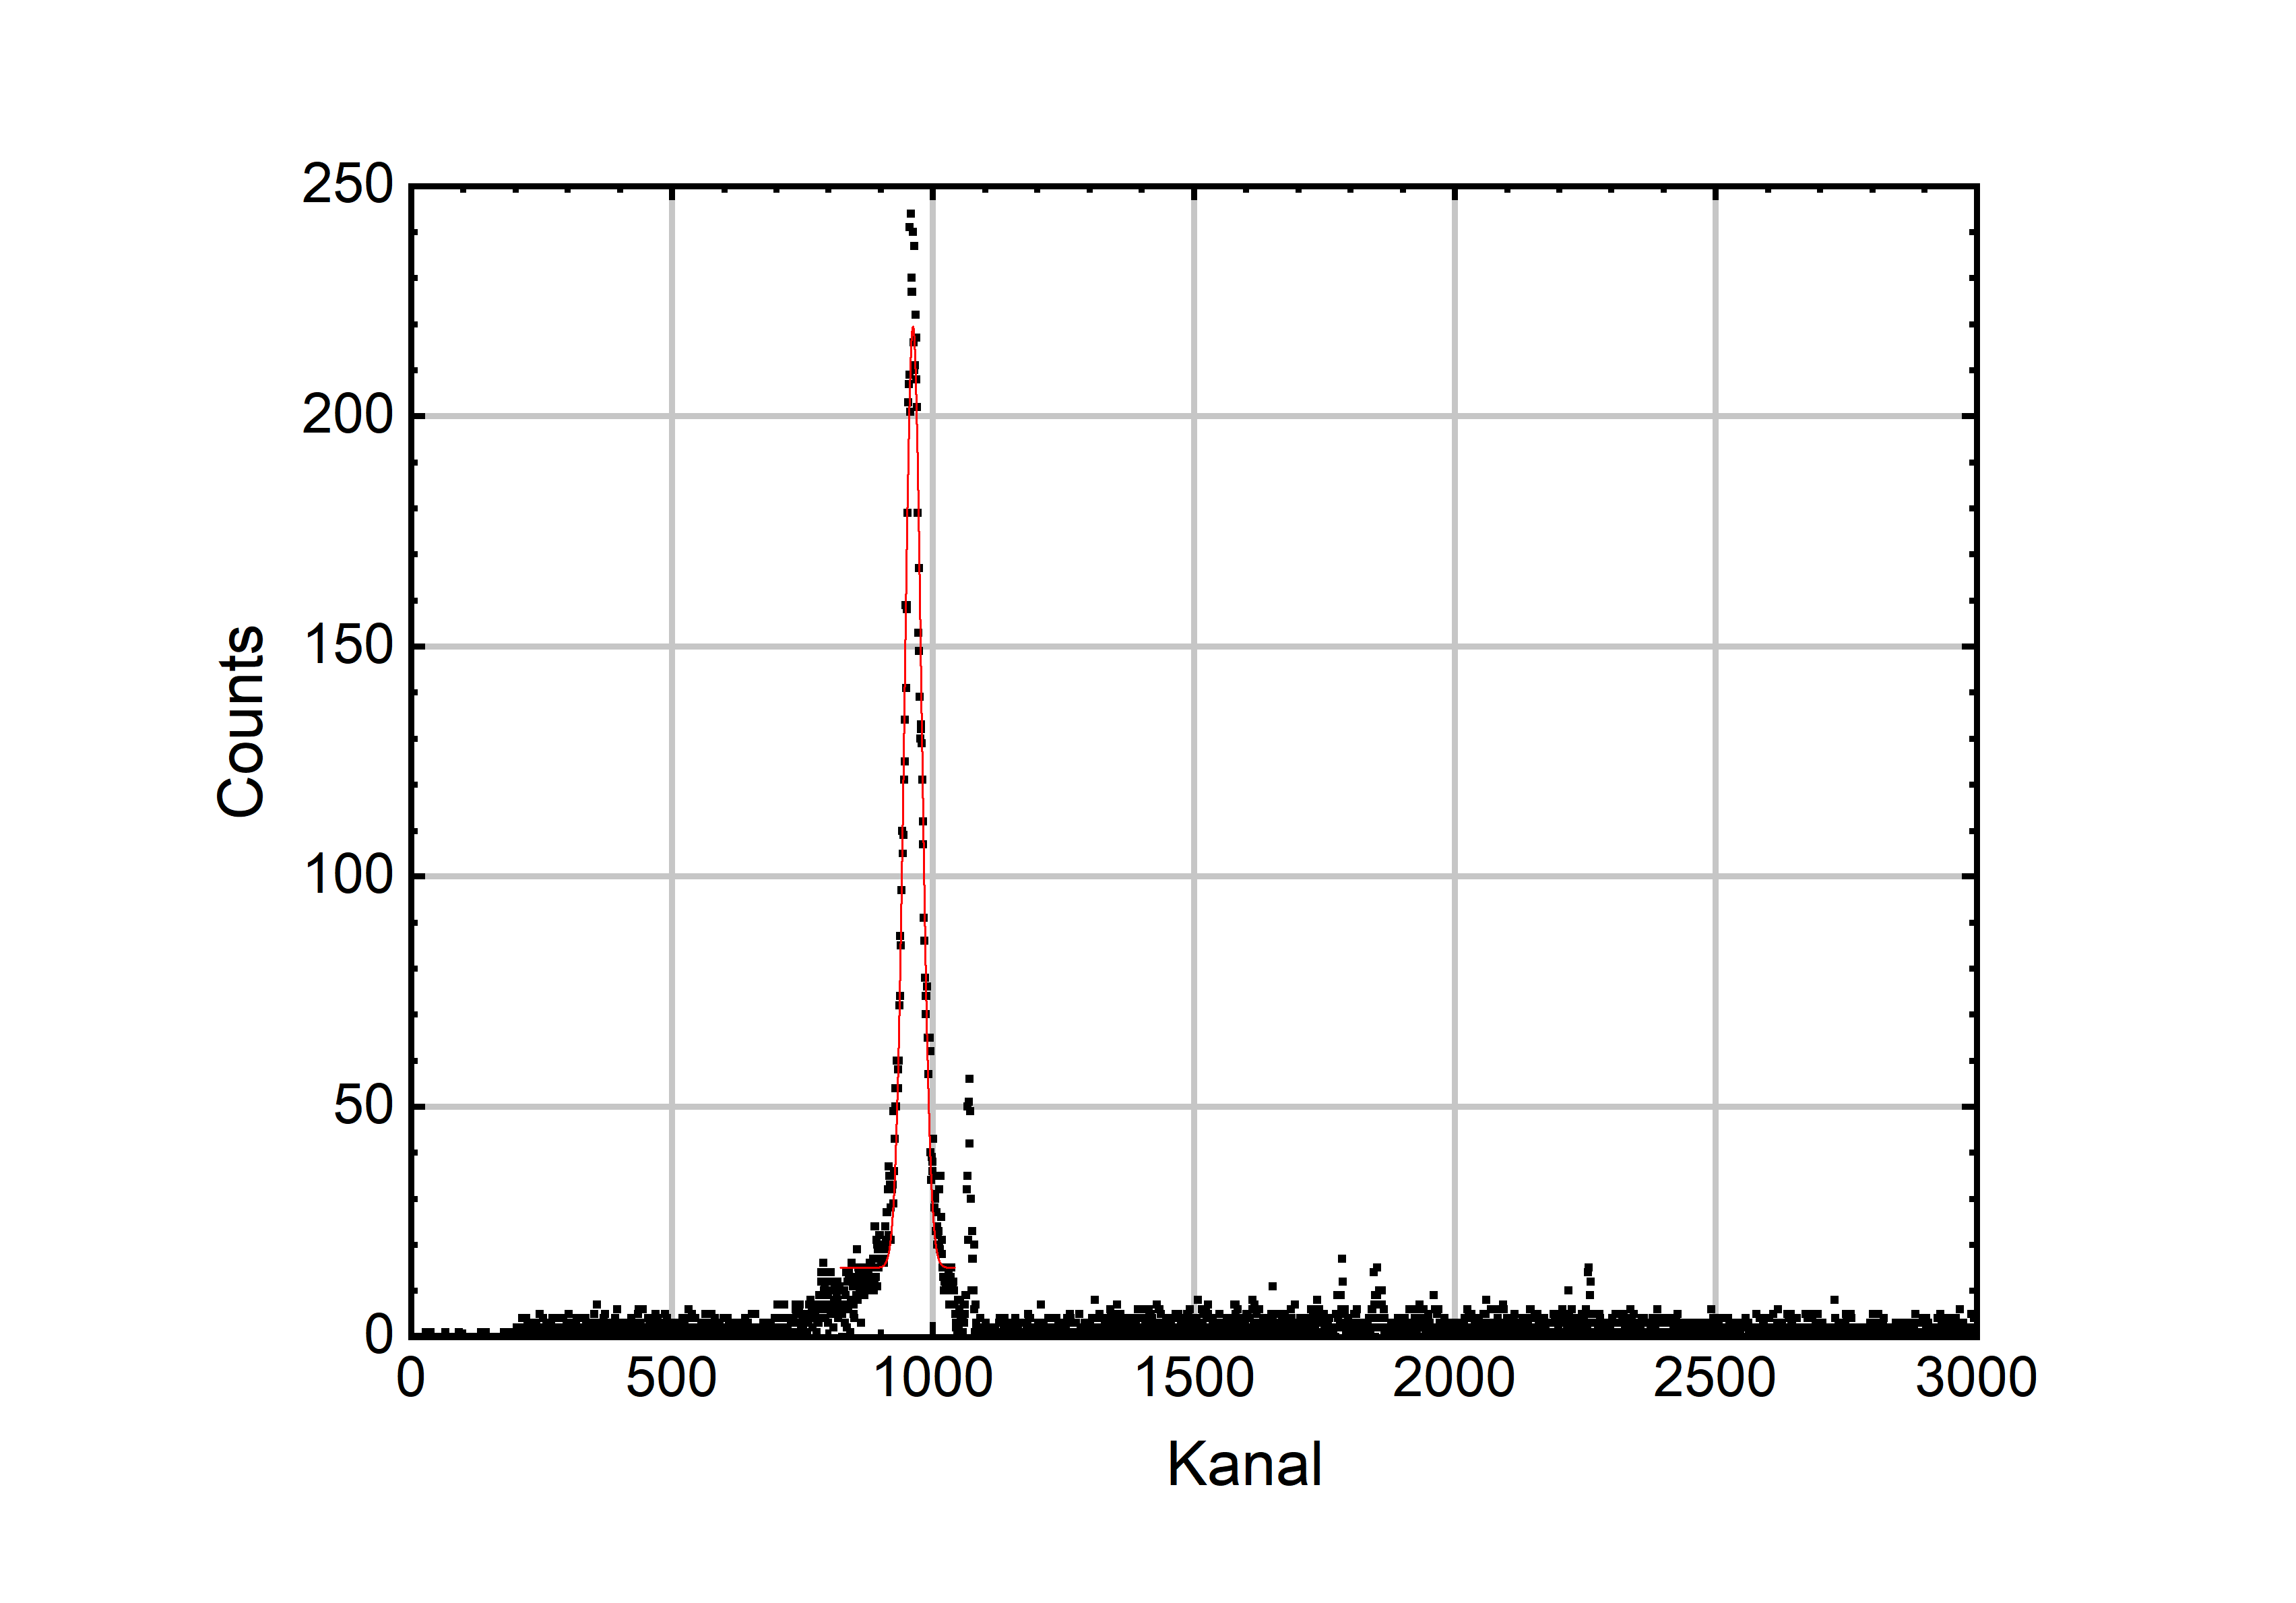
\includegraphics[scale=0.5]{zeitoptimierung}
\caption{Peakanalyse für Zeitoptimierung mittels Gauß-Fit (rot)}
\end{figure}
\\\\
Die durch die Fit-Parameter unter Berücksichtigung eines Offsets bestimmte Lage des Peaks (Kanallage) ist $K= 961,69$ und die Breite des Peaks ist $\sigma=32,2$. Somit konnte zur Bestimmung der Zählungen ein Bereich von $K \pm \sigma = 961,69 \pm 32,2$ gewählt werden. Da die Kanäle allerdings ganzzahlig sind, reduziert sich dies auf die Kanäle $929...994$. Hierbei ergibt sich:
\begin{itemize}
\item $N_{\text{g}} = 9118$
\item $N_0 = 232$
\item $N= N_{\text{g}}-N_0 = 8886$
\item $\dot{N}_{\text{g}} = \frac{N_{\text{g}}}{t} = 7,598 \, \frac{1}{\text{s}}$
\item $\dot{N}_{0} = \frac{N_{0}}{t} = 0,193 \, \frac{1}{\text{s}}$
\item $\dot{N} = \frac{N}{t} = 7,405 \, \frac{1}{\text{s}}$
\end{itemize} 
Einsetzen dieser Werte in die Gleichungen (\ref{zeit1}) und (\ref{zeit2}) liefert dann:
\begin{align}
\underline{\underline{t_{\text{opt}} \pm \Delta t_{\text{opt}} = (157,9 \pm 2,0) \, \text{s}}}
\end{align}
Das Ziel für die folgenden Messungen ist es also eine Messzeit von ca. $160$ s zu verwenden.

\subsection{Bestimmung der Energie gestreuter Photonen}
Für diesen Teilversuch ist die Photonenenergie in Abhängigkeit vom Richtungscosinus darzustellen und mit der Theorie zu vergleichen.
\\\\
Die jeweiligen Parameter der Messung für die verschiedenen Winkel $\vartheta$ sind in folgender Tabelle zusammengefasst:
\\
\begin{table}[h!]\centering
\begin{tabular}{|c|c|c|}\hline
vermessener Winkel $\vartheta$/$^{\circ}$ & Art der Messung & Messzeit t/s \\\hline
30 & mit Streukörper & 157,328 			\\\hline
30 & Nulleffekt & 157,018 			\\\hline
45 & mit Streukörper & 159,721 			\\\hline
45 & Nulleffekt & 159,577			\\\hline
60 & mit Streukörper & 158,519			\\\hline
60 & Nulleffekt & 164,873		\\\hline
75 & mit Streukörper 	& 159,853		\\\hline
75 & Nulleffekt & 162,664			\\\hline
90 & mit Streukörper & 159,125 			\\\hline
90 & Nulleffekt & 163,220		\\\hline
105 & mit Streukörper	 & 160,101		\\\hline
105 & Nulleffekt 	& 161,234		\\\hline
120 & mit Streukörper	 & 161,598	\\\hline
120 & Nulleffekt & 157,163		\\\hline
130 & mit Streukörper & 160,583			\\\hline
130 & Nulleffekt 	& 157,133		\\\hline
\end{tabular}
\caption{Parameter zur Messung der Winkelabhängigkeit der Energie}
\end{table}
\\
Außerdem wird für alle Messungen der Aluminiumstab mit $d=8$ mm verwendet. Die Unsicherheit $\Delta \vartheta$ kann mit $2^{\circ}$ angenommen werden. Die Energien werden wieder aus den Werten für die Messung mit Streukörper abzüglich des Nulleffekts über einen Gauß-Fit bestimmt. Die Kanallage kann dann wieder mittels der Kalibriergeraden in keV umgerechnet werden. Die Unsicherheit der Energie folgt wieder aus den Parametern der Energiekalibrierung. Folgende Tabelle stellt alle Ergebnisse der Messung kompakt zusammen:
\newpage
\begin{table}[h!]\centering
\begin{tabular}{|c|c|c|c|c|c|}\hline
$\vartheta$/$^{\circ}$ & $\Delta \vartheta$/$^{\circ}$ & $\mu=\cos(\vartheta)$& $\Delta \mu$ & $E$/keV & $\Delta E$/keV \\\hline
30   & 2 & 0,866 & 0,018 & 61,34 &1,26 		\\\hline
45   & 2 & 0,707 & 0,025 & 60,05 & 1,23		\\\hline
60   & 2 & 0,500 & 0,030 & 58,71 & 1,21		\\\hline
75   & 2 	& 0,259 & 0,034 & 57,31 & 1,18	\\\hline
90   & 2 & 0,000  & 0,035 & 55,82 & 1,15	\\\hline
105 & 2	& -0,259 & 0,034 & 54,24 & 1,11	\\\hline
120 & 2 & -0,500 & 0,030 & 53,10 & 1,09		\\\hline
130 & 2	& -0,643 & 0,027 & 52,31 & 1,07		\\\hline
\end{tabular}
\caption{Ergebnisse der Messung zur Winkelabhängigkeit}
\end{table}
Diese Werte sollen also nun mit der Theorie verglichen werden. Dazu sind die Messergebnisse zusammen mit den theoretischen Werten, die sich aus Gleichung (\ref{energiewinkel}) ergeben, in einem Diagramm dargestellt:
\\
\begin{figure}[h!]\centering
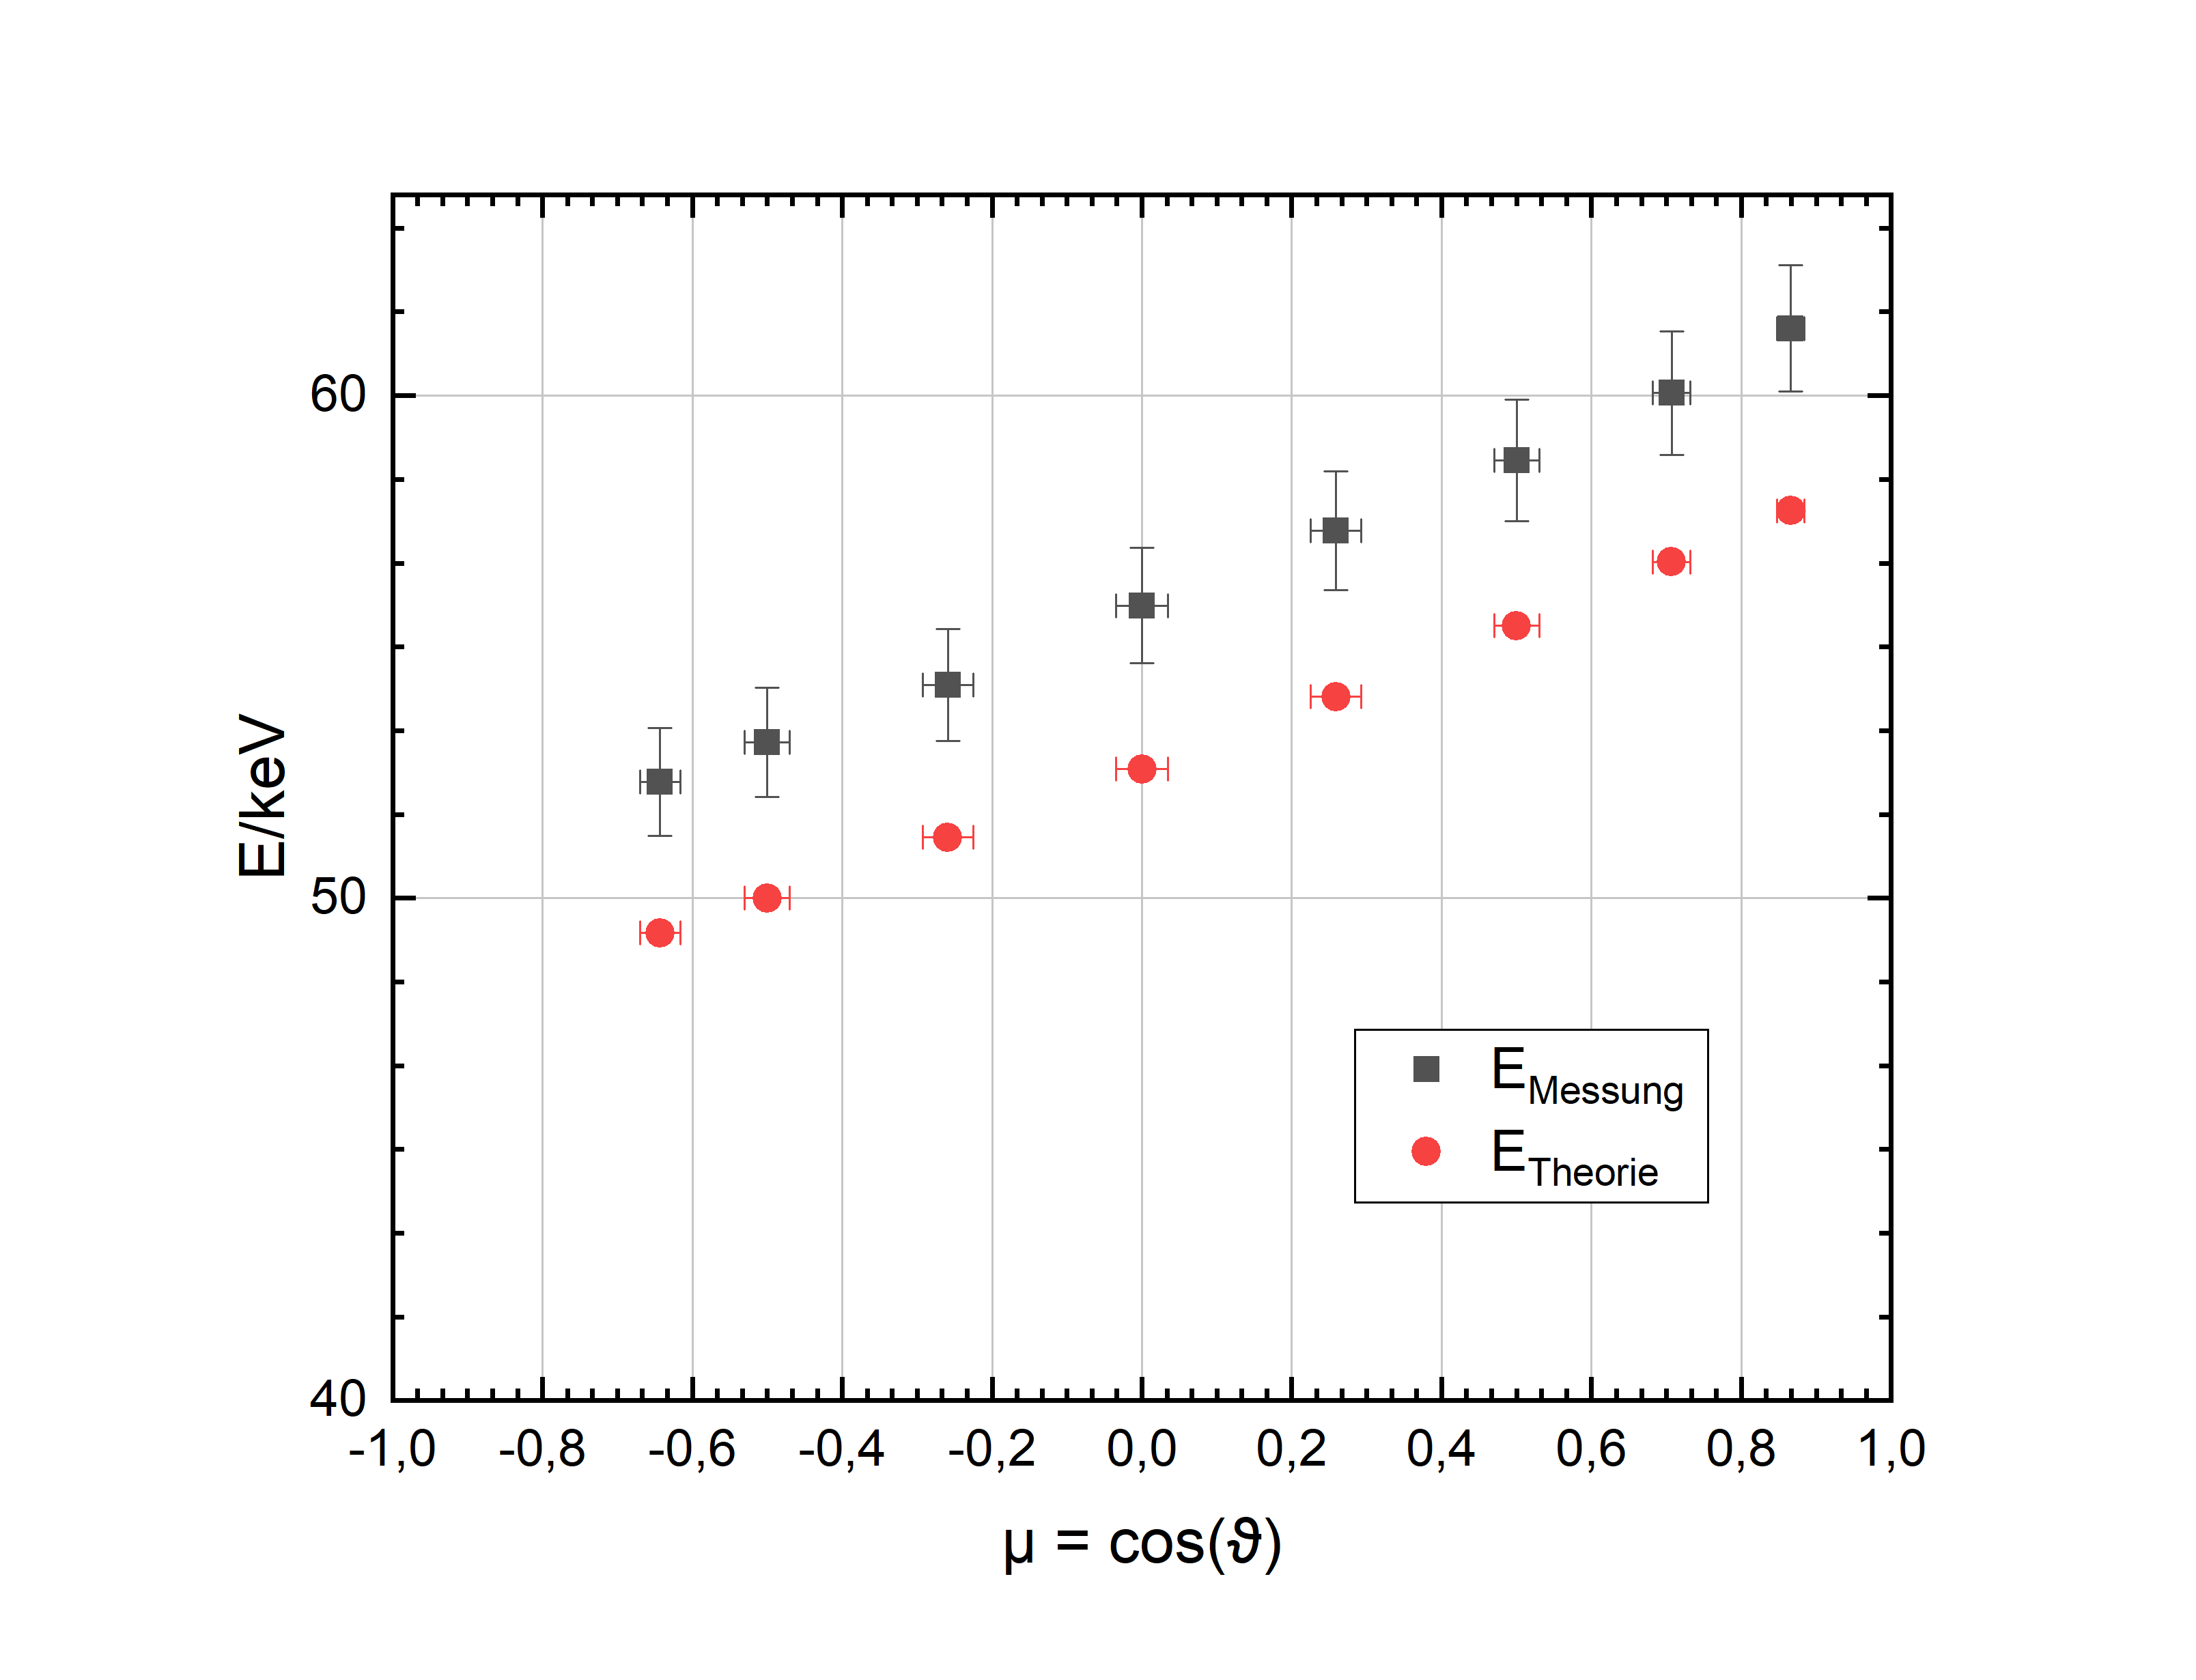
\includegraphics[scale=0.5]{vglexptheorie}
\caption{Vergleich von Theorie und Experiment für $E (\mu)$}
\end{figure}
\\
In dieser Grafik ist zu beachten, dass die Energieachse bereits bei $40$ keV beginnt. Deshalb sieht es so aus als würden Theorie und Experiment nicht sonderlich gut übereinstimmen. Wenn man allerdings den Quotienten $\frac{E_{\text{Messung}}}{E_{\text{Theorie}}}$ berechnet, liegt dieser zwischen $94$\% und $95$\%. Dies ist im Rahmen der Messung eine gute Übereinstimmung. Zudem sind die Geraden für Theorie und Experiment ziemlich parallel, sodass der prinzipielle Verlauf der Kurve gut ermittelt werden konnte. Allerdings gibt es einen deutlich erkennbaren Offset. Um diesen Sachverhalt nochmal etwas zu untermauern ist hier nochmals dieselbe Grafik mit kontinuierlichen theoretischen Werten dargestellt:
\\
\begin{figure}[h!]\centering
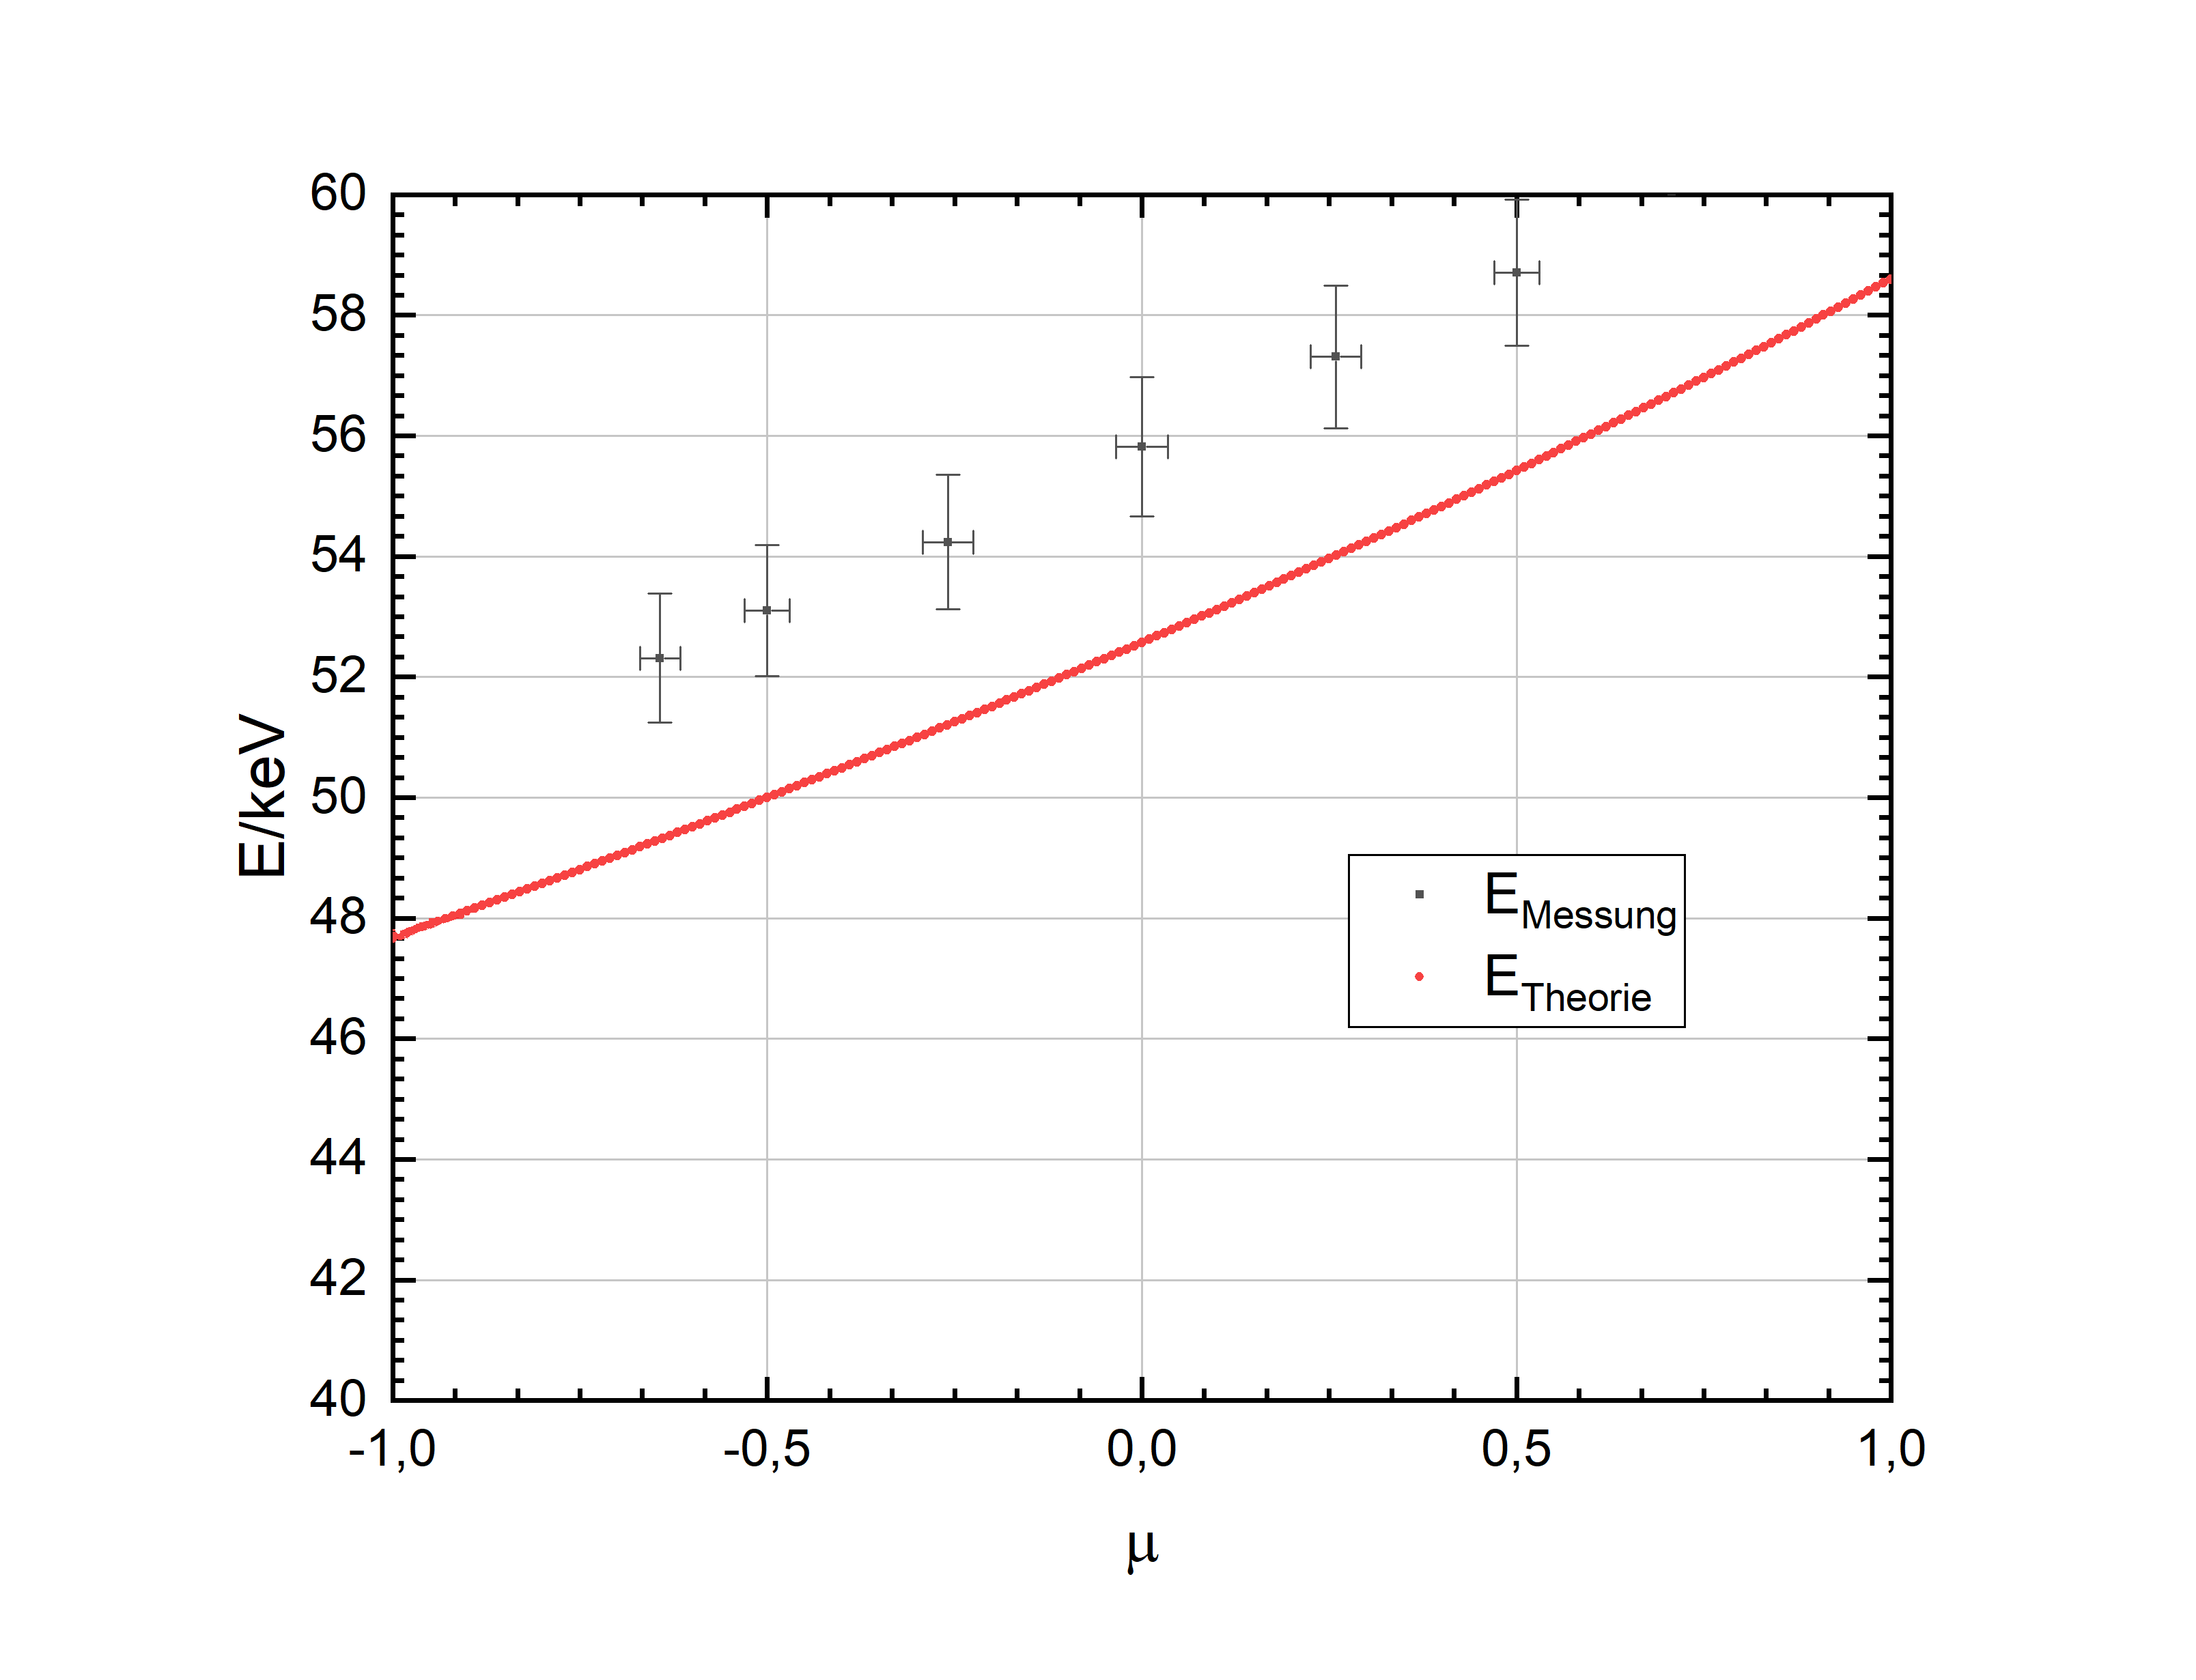
\includegraphics[scale=0.5]{vglexptheorie2}
\caption{Vergleich von Theorie und Experiment für $E (\mu)$, kontinuierlich}
\end{figure}
\\
Gründe für die vorhandene Abweichung sind, dass die Detektorakzeptanz nie bei exakt $100$\% liegen kann. Außerdem wir die Bindungsenergie vernachlässigt. Dies hat Einfluss auf die Energiebilanzierung. Für die Energiekalibrierung wurden zudem nur 6 Werte verwendet. Eine Verwendung aller Peaks würde die Genauigkeit bzw. die Übereinstimmung mit der Theorie noch verbessern.
\subsection{Bestimmung des Wirkungsquerschnitts}
In diesem Punkt der Auswertung ist die Zählrate $\dot{N}$ der Streupeaks für die verschiedenen Winkel zu bestimmen und geeignet zu skalieren. Dies soll dann mit dem Wirkungsquerschnitt nach Klein und Nishina verglichen werden. Die Zählraten können, analog zur Auswertung der Messzeitbestimmung, über Gauß-Fits bestimmt werden. Die sich so ergebenden Zählraten sind folgende:
\\\\
\begin{table}[h!]\centering
\begin{tabular}{|c|c|c|c|c|}\hline
$\vartheta/^{\circ}$  &  $\dot{N}_{\text{g}}/\text{s}^{-1}$ & $\dot{N}_{0}/\text{s}^{-1}$ & $\dot{N}/\text{s}^{-1}$ & $\dot{N}$, normiert \\\hline
30   & 33,97 & 13,62 & 20,34 & 1 		\\\hline
45   & 14,46 & 2,31 & 12,14 & 0,60		\\\hline
60   & 11,12 & 1,07 & 10,06 & 0,49 		\\\hline
75   & 8,64 	& 0,52  & 8,12 & 0,40 	\\\hline
90   & 7,33 & 0,20  & 7,13 & 0,35 	\\\hline
105 & 7,68	& 0,11 & 7,57 & 0,37 	\\\hline
120 & 8,30 & 0,10 & 8,20 & 0,40 		\\\hline
130 & 9,63 & 0,13 & 9,50 & 0,47 		\\\hline
\end{tabular}
\caption{Zählraten für verschiedene Winkel}
\end{table}
\\\\
Die verwendeten Werte für die Messzeiten sind dieselben wie in Tabelle 4. Es wurde alles auf den Wert für $\vartheta = 30^{\circ}$ normiert, da hier das Maximum der Zählrate $\dot{N}$ vorliegt.
Die Unsicherheit $\Delta \dot{N}$ ergibt sich über folgende Gleichung:
\begin{align}
\Delta \dot{N} = \sqrt{\frac{N_{\text{g}}}{t_{\text{g}}^2} + \frac{N_{0}}{t_{0}^2}}
\end{align}
\\
Diese Unsicherheiten sind hier für die einzelnen Winkel hier zusammengestellt:
\begin{table}[h!]\centering
\begin{tabular}{|c|c|c|}\hline
$\vartheta/^{\circ}$ & $\Delta \dot{N}/\text{s}^{-1}$ &  $\Delta \dot{N}$, normiert \\\hline
30   &  0,55 &0,03		\\\hline
45   & 0,32&	0,03	\\\hline
60   &  0,28&0,03	\\\hline
75   &  0,24&0,03	\\\hline
90   & 0,22&0,03	\\\hline
105 & 0,22& 0,03	\\\hline
120 &  0,23&0,03		\\\hline
130 &  0,25&0,03		\\\hline
\end{tabular}
\caption{$\Delta \dot{N}$ für verschiedene Winkel}
\end{table}
\\
Die normierten Zählraten sind nun in Abbildung 13 im Intervall von $-0,643$ bis $0,866$ für $\mu$ dargestellt. Dies entspricht gerade dem Bereich von $\cos(130^{\circ})$ bis $\cos(30^{\circ})$. Zum Vergleich wurde ebenfalls der theoretische Wert, also der normierte Wirkungsquerschnitt nach Klein-Nishina, mit eingezeichnet:
\newpage
\begin{figure}[h!]\centering
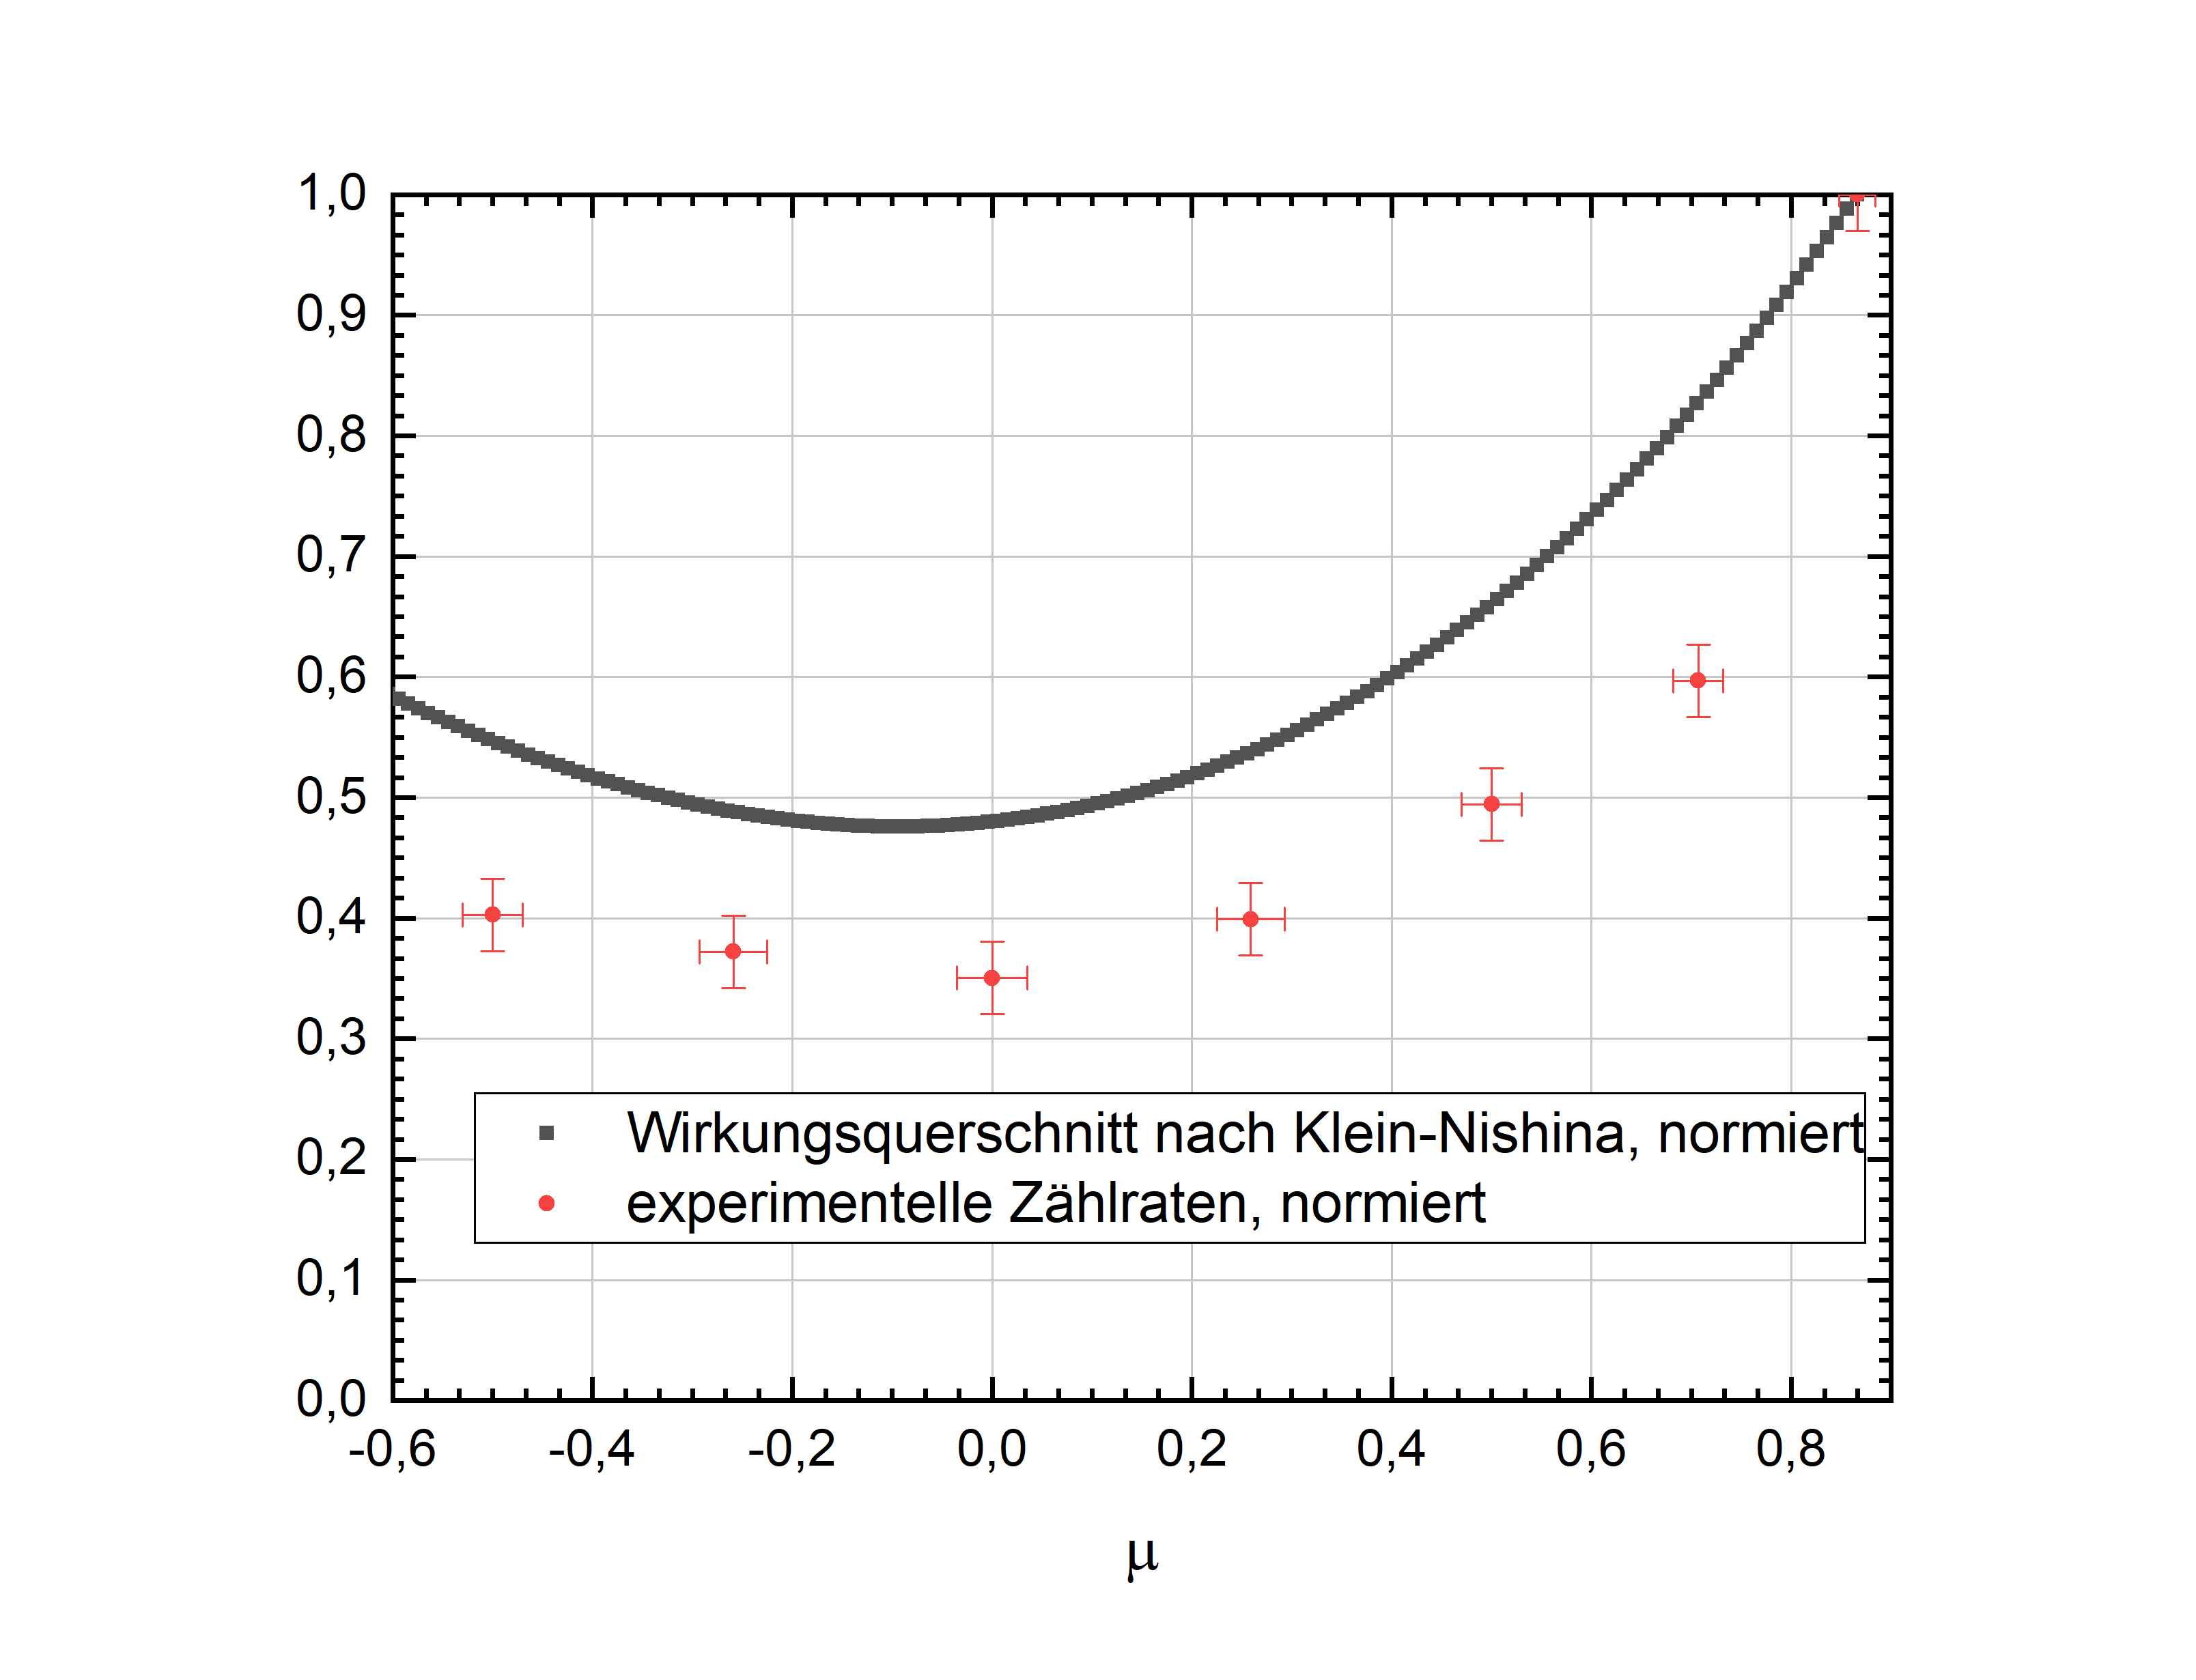
\includegraphics[scale=0.5]{wirkungsquerschnitt}
\caption{Normierte Zählrate und normierter Wirkungsquerschnitt nach Klein-Nishina}
\end{figure}
Auch hier ist, ähnlich wie in Abbildung 12, ein Offset zu erkennen. Also nur der prinzipielle Verlauf beider Kurven ist gleich.
\\\\
Auch hier liegt die Begründung in einer Betrachtung der Detektorakzeptanz , genau wie in Punkt 5.4. Die inkohärente Streufunktion ist durch die Normierung irrelevant, also diese hat keinen Einfluss auf die Abweichung.
\subsection{Einfluss des Streukörperdurchmessers}
Um die Abhängigkeit vom Streukörperdurchmesser zu untersuchen wurde die Messung für verschiedene $d$ bei minimalem Abstand von Quelle und Streukörper bei einem Winkel von $\vartheta = 60^{\circ}$ durchgeführt. Eine neue Untergrundmessung muss dafür nicht durchgeführt werden, da die Werte dafür aus der Messung zum Versuchsteil 5.4 und der Tabelle 4 entnommen werden können. Die Messzeit für die verschiedenen Durchmesser sind folgender Tabelle zu entnehmen:
\newpage
\begin{table}[h!]\centering
\begin{tabular}{|c|c|}\hline
Durchmesser $d$/mm & Messzeit t/s \\\hline
4  &  167,258		\\\hline
6  & 158,122	\\\hline
8   &  158,519	\\\hline
10   &  160,193	\\\hline
15   & 158,087	\\\hline
20 & 159,164	\\\hline
\end{tabular}
\caption{Messzeiten für verschiedene Durchmesser $d$ des Streukörpers}
\end{table}
Die benötigten Zählraten und deren Unsicherheiten ergeben sich völlig analog zum Teilversuch 5.5 und sind hier dargestellt:
\\
\begin{table}[h!]\centering
\begin{tabular}{|c|c|c|}\hline
Durchmesser $d$/mm & Zählrate $\dot{N}/\text{s}^{-1}$ & Unsicherheit $\Delta \dot{N}/\text{s}^{-1}$  \\\hline
4  &  4,40 & 0,19		\\\hline
6  & 8,03 & 0,25	\\\hline
8   &  10,06 & 0,27	\\\hline
10   &  12,92 & 0,30	\\\hline
15   & 11,40 & 0,29	\\\hline
20 & 8,94 & 0,26	\\\hline
\end{tabular}
\caption{Zählraten und deren Unsicherheit für verschiedene Durchmesser $d$ des Streukörpers}
\end{table}
\\
Die Streukörperdurchmesser wird noch als mit einer Unsicherheit $\Delta d$ behaftet angenommen. Diese wird abgeschätzt zu: $\Delta d = 0,5 $ mm.
\\\\
Somit können die Werte aus Tabelle 9 graphisch dargestellt werden:
\newpage
\begin{figure}[h!]\centering
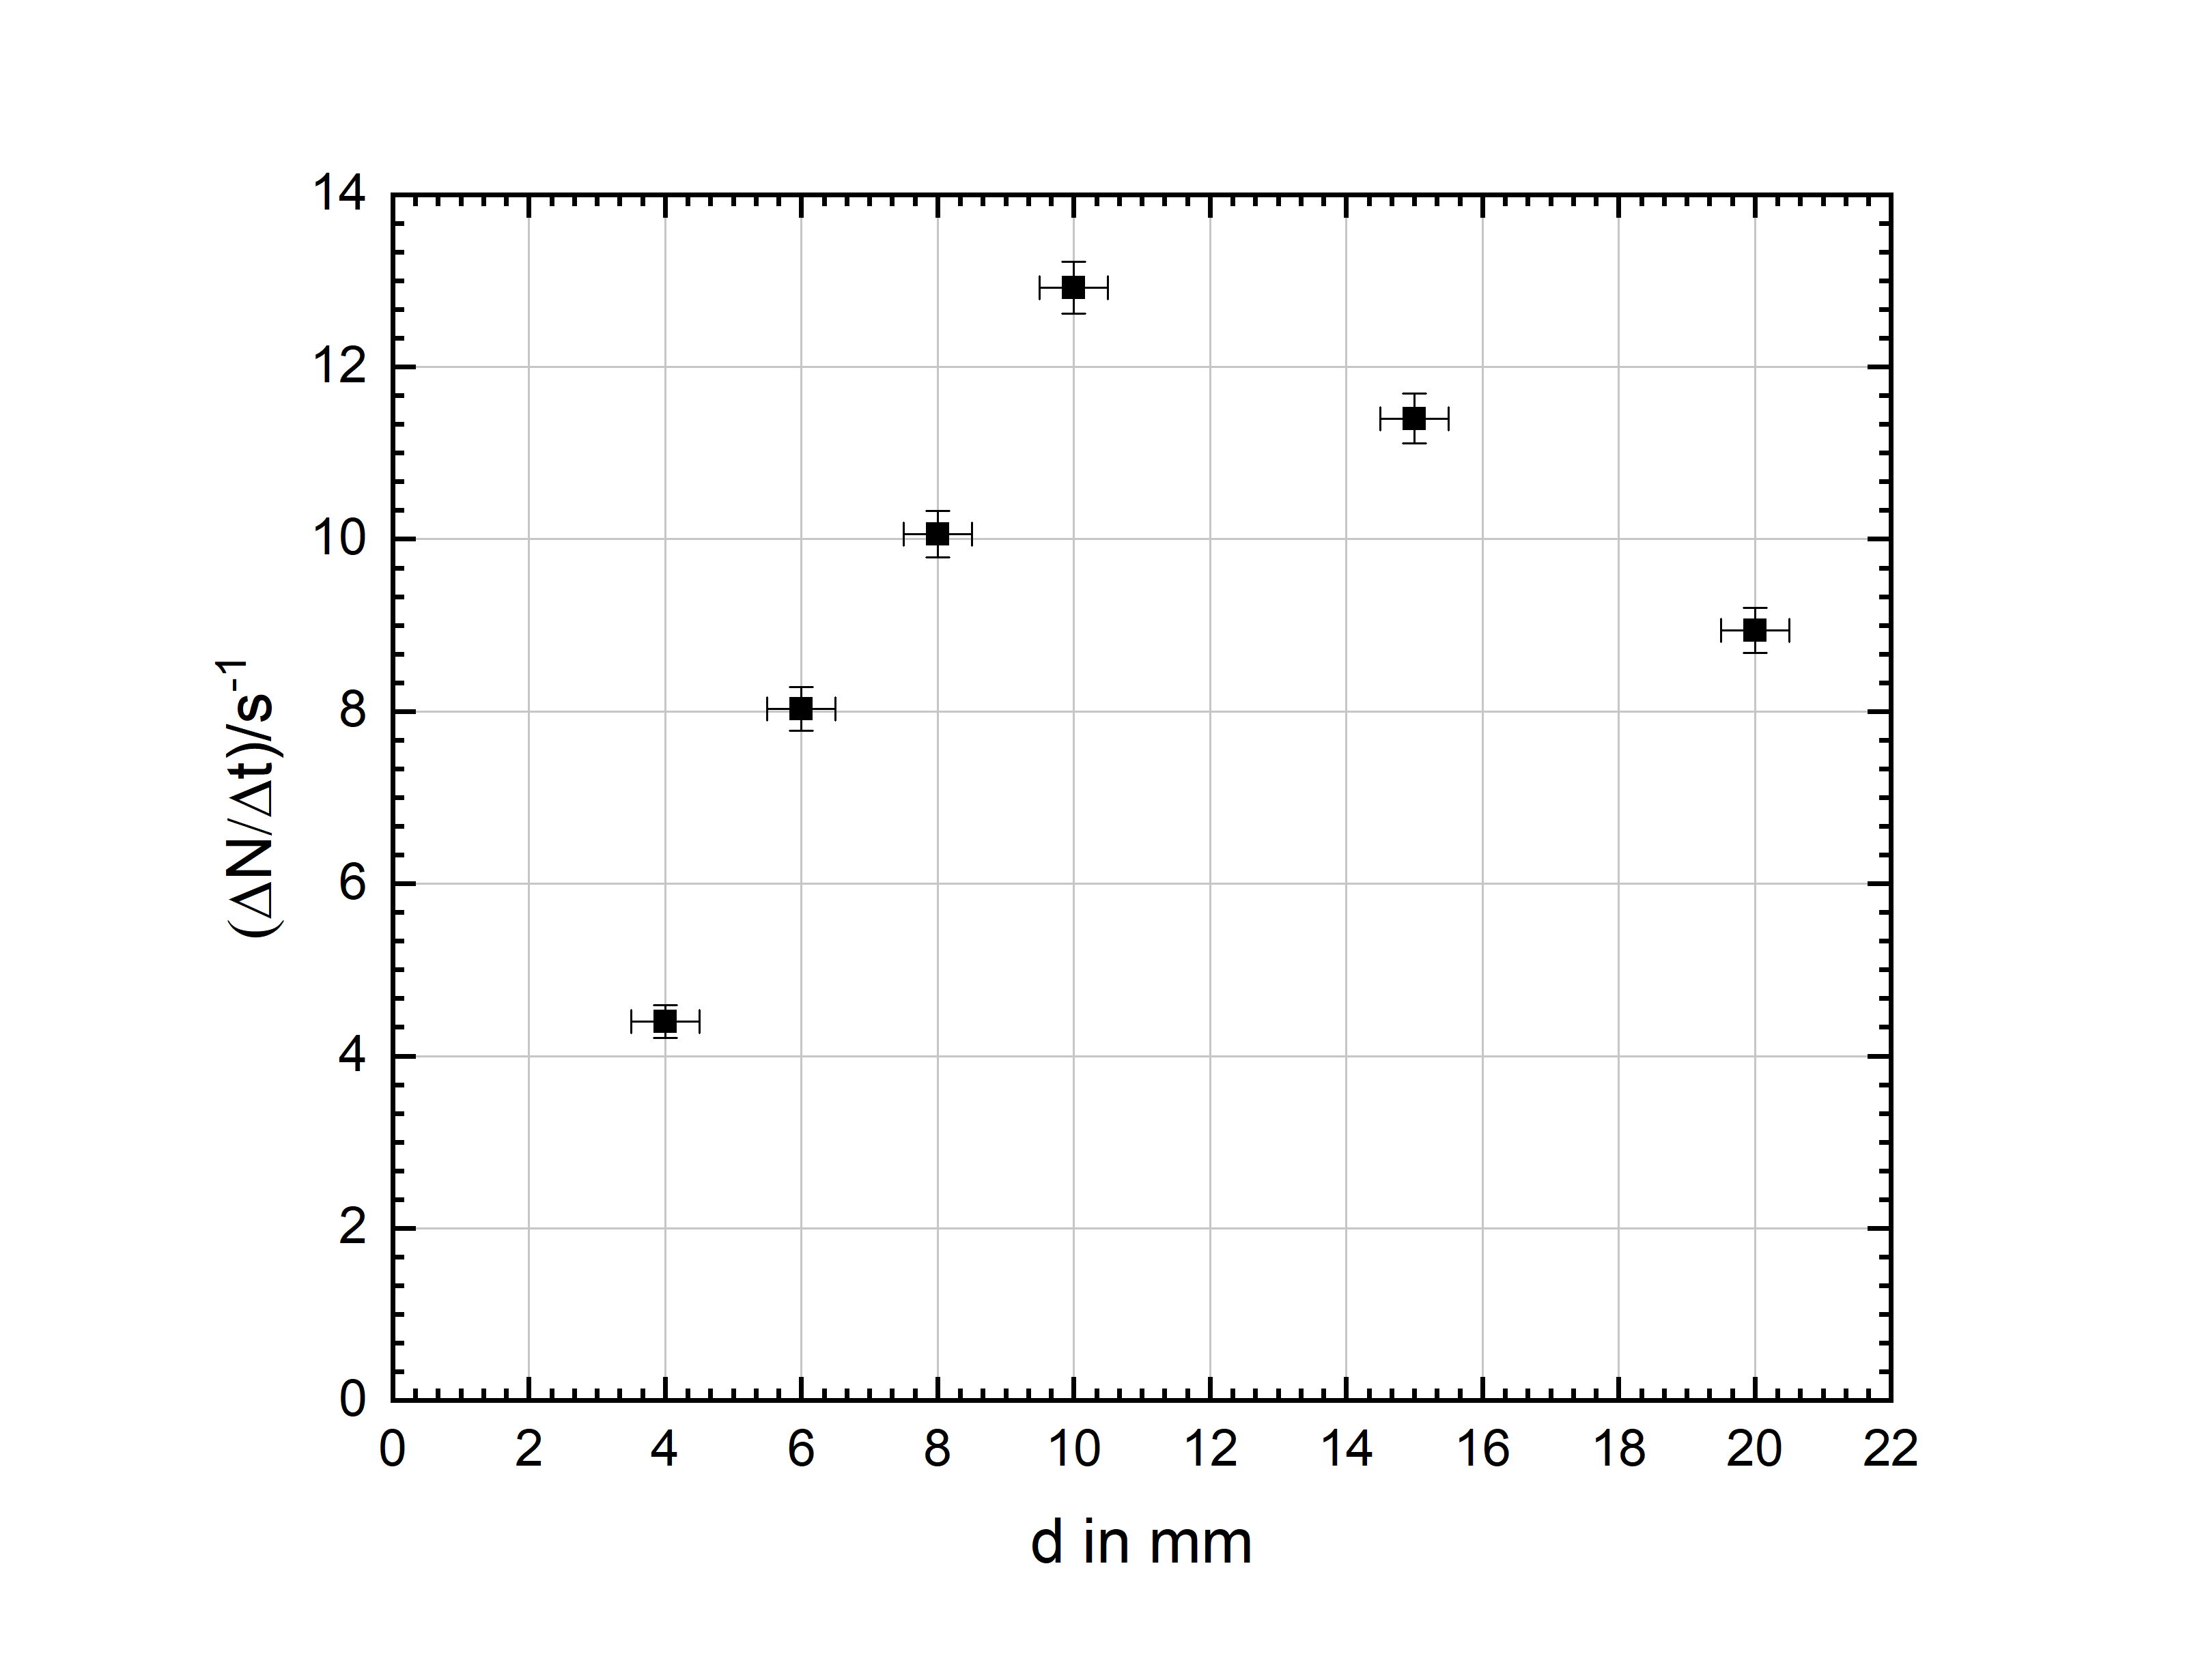
\includegraphics[scale=0.5]{durchmesser}
\caption{Zählraten in Abhängigkeit vom Streukörperdurchmesser $d$}
\end{figure}
Es ist deutlich zu erkennen, das die Zählrate für $d=10$ mm maximal ist. Für kleinere und größere Werte von $d$ werden die Zählraten geringer. Der Grund dafür ist, dass für kleine $d$ die Streuung geringer ist, im Grenzfall $d \rightarrow 0$ erhält man also das Resultat ohne Streukörper, bei dem gar keine Streuung vorliegt. Wenn also $d$ kleiner wird, erreichen immer weniger Photonen überhaupt den Detektor und die Zählrate nimmt ab. Für große $d$ nimmt aufgrund der erhöhten Dicke die Absorption der Photonen zu, sodass diese den Detektor nicht mehr erreichen können, die Zählrate sinkt also auch hier. Für das Maximum ist also das Verhältnis von der Effektivität der Streuung zur Absorption durch das Material maximal.

\subsection{Einfluss des Abstands zwischen Quelle und Streukörper}
Schließlich galt es die Abhängigkeit des Abstandes von Quelle und Streustab zu untersuchen. Die Messung wurde für den Aluminiumstab mit $d=8$ mm durchgeführt. Die Messzeiten für die einzelnen Abstände $l$ sind:
\newpage
\begin{table}[h!]\centering
\begin{tabular}{|c|c|}\hline
Abstand $l$/cm & Messzeit t/s \\\hline
4  & 164,341	\\\hline
6   &  159,110	\\\hline
8   &  166,286	\\\hline
10   & 158,271	\\\hline
\end{tabular}
\caption{Messzeiten für verschiedene Abstände $l$ zwischen Quelle und Streukörper}
\end{table}
Die Unsicherheit der Abstände kann abgeschätzt werden zu: $\Delta l = 0,25$ mm. Die durch Gauß-Fit bestimmte Kanallage und Breite des Peaks, sowie die Zählrate mit Unsicherheit finden sich in folgender Tabelle:
\\
\begin{table}[h!]\centering
\begin{tabular}{|c|c|c|c|c|}\hline
Abstand $l$/cm & $K$ des Peaks & $\sigma$ des Peaks & $\dot{N}_{\text{g}}/\text{s}^{-1}$ &  $\Delta \dot{N}_{\text{g}}/\text{s}^{-1}$\\\hline
4  & 1014,14 & 23,79 & 6,40 & 0,20	\\\hline
6   &  1012,82 & 23,57 & 5,14 & 0,18	\\\hline
8   &  1012,80 & 21,95 & 3,86 & 0,15	\\\hline
10   & 1013,13 & 19,69 & 2,79 & 0,13	\\\hline
\end{tabular}
\caption{Messzeiten für verschiedene Abstände $l$ zwischen Quelle und Streukörper}
\end{table}
\\
Es wurde abweichend von der originalen Anleitung keine Messung für $l=3$ cm durchgeführt, weshalb nur eine Normierung auf den Wert für die Gesamtzahl an Counts als Maß für die Fläche des Peaks für $l=4$ cm vorgenommen werden kann. Außerdem wurde keine Untergrundmessung durchgeführt. Deshalb ist hier bloß $\dot{N}_{\text{g}}$ dargestellt. Die normierten Counts sind hier zu finden:
\\
\begin{table}[h!]\centering
\begin{tabular}{|c|c|}\hline
Abstand $l$/cm & normierte Counts $N_{\text{norm}}$\\\hline
4  & 1	\\\hline
6   &  0,78	\\\hline
8   &  0,61	\\\hline
10   & 0,42	\\\hline
\end{tabular}
\caption{Normierte Counts für die verschiedenen Abstände $l$}
\end{table}
\\
Es kann nun das Verhalten für die Peakbreite $\sigma$ ausgewertet werden. Mit zunehmendem $l$ nimmt die Peakbreite ab. Die Untergrundzählraten für die verschiedenen Werte von $l$ unterscheiden sich untereinander. Wenn man allerdings die Annahme macht, dass sich die Untergrundzählraten nicht allzu signifikant voneinander unterscheiden, sodass die qualitative Änderung dieser in Abhängigkeit von $l$ ähnlich ist, kann man zumindest die Aussage treffen, dass die Zählrate mit zunehmendem Abstand sinkt. Selbiges gilt auch für die Gesamtzählraten, also die hier betrachteten normierten Counts.
\\\\
Die Begründung für die erste Beobachtung ist eine Betrachtung des Winkels. Es ist nicht möglich die auf den Streukörper auftreffende Photonenstrahlung vollkommen punktförmig zu realisieren. Demzufolge kann man modellhaft folgende Abbildungen betrachten:
\\
\begin{figure}[h!]\centering
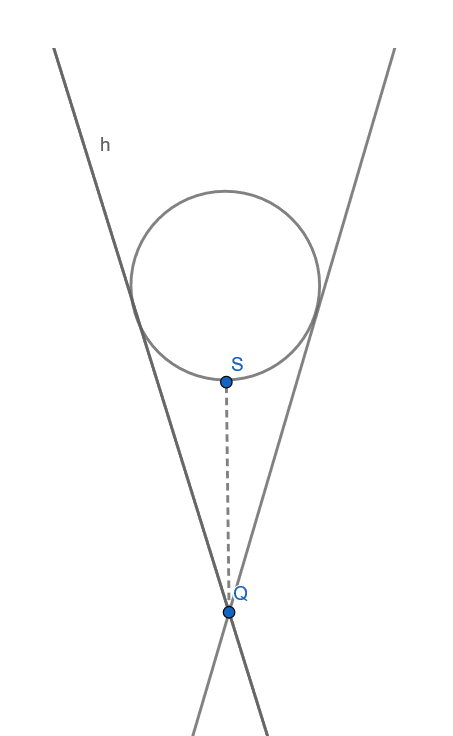
\includegraphics[scale=0.37]{abstand1}
\caption{Modell für kleine Abstände $l$}
\end{figure}
\begin{figure}[h!]\centering
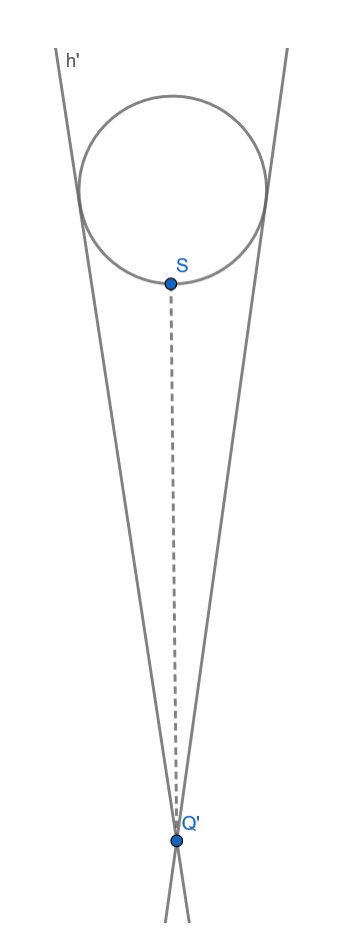
\includegraphics[scale=0.37]{abstand2}
\caption{Modell für große Abstände $l$}
\end{figure}
\newpage
Es ist an diesen Grafiken also deutlich zu erkennen, dass der Winkel zwischen der Geraden $h$ und der Strecke $\overline{\text{SQ}}$ größer ist als der Winkel zwischen $h'$ und $\overline{\text{SQ'}}$. Der Punkt $Q$ bezeichnet dabei den Ort der Quelle und $S$ denn Punkt auf dem Zylindermantel des Streukörpers, der hier die gleiche $x$-Koordinate wie der Mittelpunkt der Kreisfläche hat. Dementsprechend muss die Breite $\sigma$ für größere Winkel auch abnehmen.
\\
(Dies wurde o.B.d.A. gewählt: Man hätte auch den Mittelpunkt oder einen beliebigen anderen Punkt mit gleicher $x$-Koordinate wie $S$ wählen können, da dies nichts an dem Winkel zwischen Gerade und $\overline{\text{SQ}}$ bzw. $\overline{\text{SQ'}}$ ändert.)
\\\\
Die zweite Beobachtung kann man unter Betrachtung von Emission, Detektion, Transmission und Streuung erklären.
\\\\
Da die Quelle eines zu berücksichtigende Ausdehnung im Vergleich zur Detektorgeometrie besitzt, kann maximal nur ein Anteil $I$ der Photonen den Detektor überhaupt erreichen:
\begin{align}
I = \frac{A_{\text{S}}}{4 \, \pi \, r_{\text{SQ}}^2}
\end{align}
$A_{\text{S}}$ ist die bestrahlte Detektorfläche und $r_{\text{SQ}}$ der Abstand zwischen Quelle und Streukörper. Die Betrachtung der Emission ergibt also, dass mit zunehmendem $l$ die Zählrate abnehmen sollte.
\\\\
Der Raumwinkel, der durch den Detektor erfasst werden kann, berechnet sich aus:
\begin{align}
\Omega = \frac{A_{\text{S}}}{r_{\text{SD}}^2}
\end{align}
$r_{\text{SD}}$ ist der Abstand von Streukörper zu Detektor. Dieser wird allerdings nicht verändert. Die Betrachtung der Detektion ergibt also keine Änderung der Zählrate.
\\\\
Die Erhöhung des Abstandes zwischen Quelle und Streukörper hat zur Folge, dass sich mehr Luft zwischen diesen befindet. Es kann also eine erhöhte Streuung an Teilchen der Luft stattfinden. Außerdem wird elektromagnetische Strahlung in einem Medium exponentiell geschwächt. Diese Schwächung ist in folgender Gleichung beschrieben:
\begin{align}
S(r) = 1- e^{-r\Sigma_{t}}
\end{align}
$\Sigma_{t}$ ist die totale Wirkungsquerschnittsdichte. Diese ist materialabhängig. Im nächsten Diagramm ist zu erkennen, wie sich dieses $\Sigma$ für Luft für verschiedene Photonenenergien $E'$ verhält:
\newpage
\begin{figure}[h!]\centering
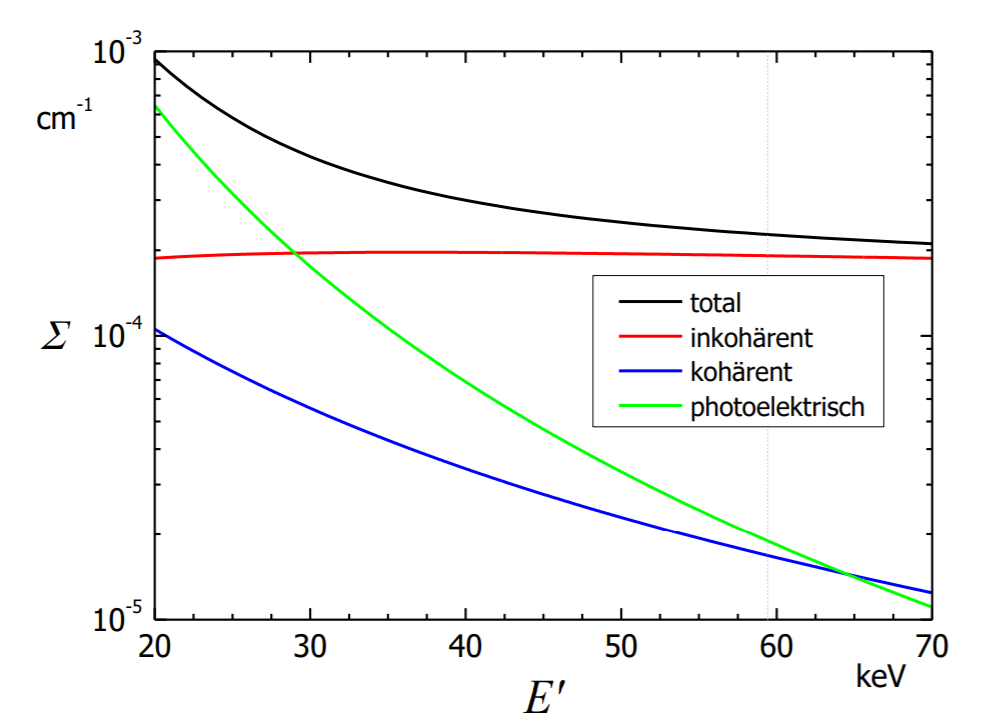
\includegraphics[scale=0.4]{sigma_luft}
\caption{Wirkungsquerschnittsdichte $\Sigma$ in Abhängigkeit der Photonenenergie $E'$, entnommen aus \cite{Anleitung}}
\end{figure}
Für inkohärente Streuung ist das $\Sigma$ für Luft also sogar annähernd konstant ist, also unabhängig von $E'$.
Hier ergibt sich also, dass die Transmission durch Luft und die Streuung an Teilchen der Luft die Zählrate mit zunehmendem Abstand senken.
\\\\
Letztendlich wird die Zählrate also vor allem durch Emission (Selbstabsorption), Transmission und Streuung vermindert, was auch experimentell (unter der Annahme, dass die Untergrundzählraten nicht signifikant voneinander abweichen) herausgefunden werden konnte. 




    % Bibliographie/Literaturverzeichnis
    \begin{thebibliography}{9}
    \bibitem{nudat}
    NuDat,
    \url{https://www.nndc.bnl.gov/nudat2/},
    21.\,Dez.~2019.
    \bibitem{Anleitung}	
    Henniger et. al.: Versuch Compton-Streuung (CS). Bestimmung der Energie gestreuter Photonen und des differentiellen Wirkungsquerschnitts des Streuprozesses in Abhängigkeit des Streuwinkels . 2019.
\bibitem{feynman}
    Feynman-Diagramm,
    \url{https://feynman.aivazis.com/},
    22.\,Dez.~2019.
\end{thebibliography}
% Ende Dokument

\end{document}
